\documentclass[titlepage, a4paper, reqno, openany]{report}
%%%%%%%%%%%%%%%%%%%%%%%%%%%%%%%%%%%%%%%%%%%%%%%%%%%%%%%%%%%%%%%%%%%%%
% Comment out things that are not used
%
%
%%%%%%%%%%%%%%%%%%%%%%%%%%%%%%%%%%%%%%%%%%%%%%%%%%%%%%%%%%%%%%%%%%%%%
%%%%%%%%%%%%%%%%%%%%%%%%%%%%%%%%%%%%%%%%%%%%%%%%%%%%%%%%%%%
%%			PREAMBLE LATEX GENERAL USE
%%	author: sergio manuel salazar dos santos
%%	email: sergio.salazar.santos@gmail.com
%%	Comment:
%%		Stable, no issues found yet.
%%		Note sequence is importante, and beware of clatching packages.
%%
%%		review: 24032023
%%
%%%%%%%%%%%%%%%%%%%%%%%%%%%%%%%%%%%%%%%%%%%%%%%%%%%%%%%%%%%
% preloaded:
% longtable, xcolor, graphicx, booktabs, caption, csquotes, hyperref,
% calc, listings, datetime2, siunitx, geometry, enumitem
%%%%%%%%%%%%%%%%%%%%%%%%%%%%%%%%%%%%%%%%%%%%%%%%%%%%%%%%%%%
\usepackage{etoolbox}
\usepackage{xparse}
%%%%%%%%%%%%%%%%%%%%%%%%%%%%%%%%%%%%%%%%%%%%%%%%%%%%%%%%%%%
\usepackage[T1]{fontenc}
%\usepackage{inputenc}
\usepackage[utf8]{inputenc}
%\usepackage[latin1]{inputenc} % bad behavior
%%%%%%%%%%%%%%%%%%%%%%%%%%%%%%%%%%%%%%%%%%%%%%%%%%%%%%%%%%%
\usepackage{lmodern}
\usepackage[portuguese]{babel}
%%%%%%%%%%%%%%%%%%%%%%%%%%%%%%%%%%%%%%%%%%%%%%%%%%%%%%%%%%%
\usepackage{scrbase} % Required for handling language-dependent names of sections/document elements
\usepackage{scrhack} % Loads fixes for various packages
\usepackage{longtable} % Required for tables that span multiple pages 
\usepackage[dvipsnames, svgnames, table]{xcolor} % Required for specifying custom colours
\usepackage{graphics}
\usepackage{booktabs} % Required for better table rules, enhances the quality of tables in LaTeX
\usepackage[autostyle=true]{csquotes}
\usepackage{calc} % \setcounter, \addtocounter, \setlength, and \addtolength
%%%%%%%%%%%%%%%%%%%%%%%%%%%%%%%%%%%%%%%%%%%%%%%%%%%%%%%%%%%
\usepackage{listings} % \begin{lstlisting}[language=Python] \end{lstlisting} or \lstinputlisting[caption=<name>, language=Octave, firstline=2, lastline=12]{<filename>.m}, personalize \lstdefinestyle{<name>}{<parameter>}
%\usepackage{listingsutf8}
%%%%%%%%%%%%%%%%%%%%%%%%%%%%%%%%%%%%%%%%%%%%%%%%%%%%%%%%%%%
\RequirePackage[calc, portuguese]{datetime2} % For date format
\usepackage{siunitx} % SI units system
\usepackage{paralist} % Provides enumerate and itemize environments
\usepackage{makeidx} % Standard package for creating indexes
\usepackage{titlepic}
\usepackage{ragged2e}
\usepackage{blindtext}
\usepackage{hyphsubst}
\usepackage[top=2cm,left=1.5cm,right=1.2cm,bottom=2cm]{geometry}
\usepackage{graphicx}
\usepackage[graphicx]{realboxes}
\usepackage{hyphenat}
\usepackage{color,colortbl}
\usepackage[dvipsnames, svgnames, table]{xcolor}
%%%%%%%%%%%%%FIXED ORDER%%%%%%%%%FIXED ORDER%%%%%%%%%%%%%%
\usepackage[acronym, toc, shortcuts, acronymlists={hidden}, nopostdot, nogroupskip, nonumberlist, automake=immediate]{glossaries} % for lists of terms, acronyms and symbols
%\usepackage[nottoc]{tocbibind}
%%%%%%%%%%%%%%%%%%%%%%%%%%%%%%%%%%%%%%%%%%%%%%%%%%%%%%%%%%%
\usepackage[markcase=used]{scrlayer-scrpage}
%%%%%%%%%%%%%%%%%%%%%%%%%%%%%%%%%%%%%%%%%%%%%%%%%%%%%%%%%%%


%%%%%%%%%%%%%%%%%%%%%%%%%%%%%%%%%%%%%%%%%%%%%%%%%%%%%%%%%%
% FYI, the following packages are preloaded with the document class:
% longtable, xcolor, graphicx, booktabs, caption, csquotes, hyperref,
% calc, listings, datetime2, siunitx, geometry, enumitem
%%%%%%%%%%%%%%%%%%% extra packages %%%%%%%%%%%%%%%%%%%%%%%
\usepackage{commath, amsmath}		% the principal package in the AMS-LATEX distribution $<math>$ \(<math>\) \[<math>\] \begin{gather*} \end{gather*} \begin{math} \end{math} \begin{displaymath} \end{displaymath} \begin{equation} \end{equation}
\usepackage{amsfonts}				% extended set of fonts for use in mathematics
\usepackage{amssymb}				% adds new symbols to be used in math mode
\usepackage{MnSymbol}				% adds new symbols to be used in math mode
%\usepackage{derivative}			% derivative
%\usepackage[italicdiff]{physics} 	% physic
%%%%%%%%%%%%%%%%%%%%%%%%%%%%%%%%
%%% Choice extarrows or extpfeil
%\usepackage{extarrows}				% adds new arrow symbols to be used in math mode
\usepackage{extpfeil}				% adds new arrow symbols to be used in math mode
%%%%%%%%%%%%%%%%%%%%%%%%%%%%%%%%
\usepackage{mathrsfs}				% math fonts, e.g., Laplace
\usepackage{float}					% provides the H float modifier option
\usepackage{multirow}				% tables \multirow command
\usepackage{subcaption}				% enables subfigures
\usepackage{lscape}					% for landscape mode
\usepackage{verbatim}				% new verbatim environment, \begin{comment} \end{comment}, \verbatiminput
%%%%%%%%%%%%%%%%%%%%%%%%%%%%%%%%%%%%%%%%%%%%%%%%%%%%%%%%%%
%add extra packages if needed here
%%%%%%%%%%%%%%%%%%%%%%%%%%%%%%%%%%%%%%%%%%%%%%%%%%%%%%%%%%
\usepackage[font=small, labelfont=bf]{caption} % caption for figures and tables
\usepackage{hyphenat}
\usepackage{multicol}
\usepackage{makecell}
\usepackage{array}
\usepackage{tabularx}
\usepackage[export]{adjustbox}
\usepackage{eurosym}
%%%%%%%%%%%%%%%%%%%%%%%%%%%%%%%%
%%% Choice enumitem or enumerate
\usepackage{enumitem}
%\usepackage{enumerate}
%%%%%%%%%%%%%%%%%%%%%%%%%%%%%%%%
\usepackage{setspace}
\usepackage{lipsum}
\usepackage{moreverb}
\usepackage{rotating}
\usepackage{romannum}
%%%%%%%%%%%%%%%%%%%%%%%%%%%%%%%%
%%% Choice biblatex or babelbib
%\usepackage{biblatex} % \addbibresource{<location>} and \printbibliography
\usepackage[portuguese]{babelbib} % \bibliographystyle{<style>} and \bibliography{<location>}, remove '@' to comment out in bib file
\usepackage[toc, page]{appendix} % \appendix then \include{<location file>}
%%%%%%%%%%%%%%%%%%%%%%%%%%%%%%%%
\usepackage{url}
\usepackage[hidelinks]{hyperref}
\usepackage[hyperpageref]{backref}
%%%%%%%%%%%%%%%%%%%%%%%%%%%%%%%%%%%%%%%%%%%%%%%%%%%%%%%%%%
\usepackage{pgfgantt}
\usepackage{tikz} % \begin{tikzpicture} \end{tikzpicture}
\usetikzlibrary{cd} % \begin{tikzcd} \end{tikzcd}
\usepackage{circuitikz} % \begin{circuitikz} \draw \end{circuitikz}
%%%%%%%%%%%%%%%%%%%%%%%%%%%%%%%%%%%%%%%%%%%%%%%%%%%%%%%%%%
\usepackage[tickmarkheight=5em,textwidth=\marginparwidth,textsize=small]{todonotes} % insert small notes [\todo[inline]{<message>} and \listoftodos]
%%%%%%%%%%%%%%%%%%%%%%%%%%%%%%%%%%%%%%%%%%%%%%%%%%%%%%%%%%%
\usetikzlibrary{cd, matrix, shapes.geometric, arrows, trees, positioning, calc}
\graphicspath{{graphic}{graphic/logo}{graphic/icon}{image}{image/logo}{image/icon}{figure}{figure/logo}{figure/icon}} 	% Specifies where to look for included images
%%%%%%%%%%%%%%%%%%%%%%%%%%%%%%%%%%%%%%%%%%%%%%%%%%%%%%%%%%%
\bibliographystyle{babplain}
%\bibliographystyle{plain}
%\bibliographystyle{ieeetr}
%%%%%%%%%%%%%%%%%%%%%%%%%%%%%%%%%%%%%%%%%%%%%%%%%%%%%%%%%%%
%%%%%%%%%%%%%%%%%%%%%%%%%%%%%%%%%%%%%%%%%%%%%%%%%%%%%%%%%%%%%%%%%%%%%
							%%%COMMAND%%%
%%%%%%%%%%%%%%%%%%%%%%%%%%%%%%%%%%%%%%%%%%%%%%%%%%%%%%%%%%%%%%%%%%%%%
\newglossary[algh]{hidden}{acrh}{acnh}{Hidden Acronyms}
%%%%%%%%%%%%%%%%%%%%%%%%%%%%%%%%%%%%%%%%%%%%%%%%%%%%%%%%%%%%%%%%%%%%%
\def\thesection{\arabic{section}} % \alph or \arabic or \roman
%%%%%%%%%%%%%%%%%%%%%%%%%%%%%%%%%%%%%%%%%%%%%%%%%%%%%%%%%%%%%%%%%%%%%
\newcommand{\emptyline}{\hfill \vspace{\baselineskip} \newline}
\newcommand{\emptyspace}[1]{\hfill \vspace{#1} \newline}
\newcommand{\minipagespace}[1]{\hfill \newline \vspace{#1} \newline}
\newcommand{\tablespace}[1]{\hfill \vspace{#1} \newline}
\newcommand{\figurespace}[1]{\hfill \vspace{#1} \newline}
\newcommand{\graphicspace}[1]{\hfill \vspace{#1} \newline}
\newcommand{\listingspace}[1]{\hfill \vspace{#1} \newline}
\newcommand{\equationspace}[1]{\hfill \vspace{#1} \newline}
%%%%%%%%%%%%%%%%%%%%%%%%%%%%%%%%%%%%%%%%%%%%%%%%%%%%%%%%%%%%%%%%%%%%%
\newcolumntype{L}[1]{>{\raggedright\arraybackslash}p{#1}}
\newcolumntype{C}[1]{>{\centering\arraybackslash}p{#1}}
\newcolumntype{R}[1]{>{\raggedleft\arraybackslash}p{#1}}
%%%%%%%%%%%%%%%%%%%%%%%%%%%%%%%%%%%%%%%%%%%%%%%%%%%%%%%%%%%%%%%%%%%%%
\newcommand\acrfullr[2][]{\acrshort[#1]{#2} (\acrlong[#1]{#2})}
%%%%%%%%%%%%%%%%%%%%%%%%%%%%%%%%%%%%%%%%%%%%%%%%%%%%%%%%%%%%%%%%%%%%%
\def\mcirc{\mathbin{\scalerel*{\bigcirc}{t}}}
\def\msquare{\mathord{\scalerel*{\Box}{gX}}}
\def\ce{\mathrm{e}}
%%%%%%%%%%%%%%%%%%%%%%%%%%%%%%%%%%%%%%%%%%%%%%%%%%%%%%%%%%%%%%%%%%%%%
\definecolor{codegreen}{rgb}{0,0.6,0}
\definecolor{codegray}{rgb}{0.5,0.5,0.5}
\definecolor{codepurple}{rgb}{0.58,0,0.82}
\definecolor{codebackcolour}{rgb}{0.95,0.95,0.92}
\definecolor{light-gray}{gray}{0.95}
\definecolor{lightgray}{rgb}{.9,.9,.9}
\definecolor{mypink1}{rgb}{0.858, 0.188, 0.478}
\definecolor{mypink2}{RGB}{219, 48, 122}
\definecolor{mypink3}{cmyk}{0, 0.7808, 0.4429, 0.1412}
\definecolor{mygray}{gray}{0.6}
%%%%%%%%%%%%%%%%%%%%%%%%%%%%%%%%%%%%%%%%%%%%%%%%%%%%%%%%%%%%%%%%%%%%%
\lstdefinestyle{CLanguageStyle}{
    belowcaptionskip=1\baselineskip,
    backgroundcolor=\color{codebackcolour},   
    commentstyle=\color{codegreen},
    keywordstyle=\color{magenta},
    numberstyle=\tiny\color{codegray},
    stringstyle=\color{codepurple},
    basicstyle=\ttfamily\footnotesize,
    breakatwhitespace=false,         
    breaklines=true,                 
    keepspaces=true,                 
    numbers=left,       
    numbersep=5pt,                  
    showspaces=false,                
    showstringspaces=false,
    showtabs=false,                  
    tabsize=2,
}
%%%%%%%%%%%%%%%%%%%%%%%%%%%%%%%%%%%%%%%%%%%%%%%%%%%%%%%%%%%%%%%%%%%%%
\setlistdepth{12}
\newlist{enumitem}{enumerate}{12}
\setlist[enumitem,1]{label=\roman*)}
\setlist[enumitem,2]{label=\alph*)}
\setlist[enumitem,3]{label=\arabic*)}
\setlist[enumitem,4]{label=(\roman*)}
\setlist[enumitem,5]{label=(\alph*)}
\setlist[enumitem,6]{label=(\arabic*)}
\setlist[enumitem,7]{label=\roman*)}
\setlist[enumitem,8]{label=\alph*)}
\setlist[enumitem,9]{label=\arabic*)}
\setlist[enumitem,10]{label=(\roman*)}
\setlist[enumitem,11]{label=(\alph*)}
\setlist[enumitem,12]{label=(\arabic*)}
%%%%%%%%%%%%%%%%%%%%%%%%%%%%%%%%%%%%%%%%%%%%%%%%%%%%%%%%%%%%%%%%%%%%%
\renewcommand{\labelitemi}{$\bullet$}
\renewcommand{\labelitemii}{$\cdot$}
\renewcommand{\labelitemiii}{$\diamond$}
\renewcommand{\labelitemiv}{$\ast$}
%%%%%%%%%%%%%%%%%%%%%%%%%%%%%%%%%%%%%%%%%%%%%%%%%%%%%%%%%%%%%%%%%%%%%
\tikzstyle{startstop} = [rectangle, rounded corners, 
minimum width=3cm, 
minimum height=1cm,
text centered, 
draw=black, 
fill=red!30]

\tikzstyle{io} = [trapezium, 
trapezium stretches=true, % A later addition
trapezium left angle=70, 
trapezium right angle=110, 
minimum width=3cm, 
minimum height=1cm, text centered, 
draw=black, fill=blue!30]

\tikzstyle{process} = [rectangle, 
minimum width=3cm, 
minimum height=1cm, 
text centered, 
text width=3cm, 
draw=black, 
fill=orange!30]

\tikzstyle{decision} = [diamond, 
minimum width=3cm, 
minimum height=1cm, 
text centered, 
draw=black, 
fill=green!30]

\tikzstyle{arrow} = [thick,->,>=stealth]

\tikzstyle{RECTANGLE_2} = [rectangle, draw, text width=5em, text centered, rounded corners, minimum height=4em]

\tikzstyle{RECTANGLE_3} = [rectangle, rounded corners, minimum width=3cm, minimum height=1cm,text centered, draw=black, fill=red!80]

\tikzstyle{RECTANGLE_4} = [rectangle, draw, fill=blue!20, text width=3cm, text centered, minimum height=4em]

\tikzstyle{RECTANGLE_5} = [rectangle, minimum width=3cm, minimum height=1cm, text centered, text width=3cm]

\tikzstyle{RECTANGLE_6} = [rectangle, draw, fill=blue!20, text width=5em, text centered, rounded corners, minimum height=4em]

\tikzstyle{RECTANGLE_7} = [rectangle, draw, fill=blue!20, text width=5em, text centered, rounded corners, minimum height=4em]

\tikzstyle{RECTANGLE_8} = [rectangle, draw, align=left, fill=blue!20]

\tikzstyle{RECTANGLE_1} = [rectangle, rounded corners, minimum width=1cm, minimum height=1cm,text centered, draw=black, fill=green!30]

\tikzstyle{DIAMOND_1} = [diamond, draw, fill=blue!20, text width=4.5em, text badly centered, node distance=4cm, inner sep=0pt]

\tikzstyle{DIAMOND_2} = [diamond, minimum width=3cm, minimum height=1cm, text centered, draw=black, fill=green!30]

\tikzstyle{DIAMOND_3} = [diamond, draw, text width=4.5em, text badly centered, node distance=3cm, inner sep=0pt]

\tikzstyle{DIAMOND_4} = [diamond, draw, fill=blue!20, text width=4.5em, text badly centered, node distance=3cm, inner sep=0pt]

\tikzstyle{DIAMOND_5} = [diamond, draw, fill=blue!20, text width=4.5em, text badly centered, node distance=3cm, inner sep=0pt]

\tikzstyle{DIAMOND_6} = [diamond, draw, fill=blue!20, text width=4.5em, text badly centered, node distance=4cm, inner sep=0pt]

\tikzstyle{DIAMOND_7} = [diamond, draw, align=left, fill=blue!20]

\tikzstyle{ELLIPSE_1} = [draw, ellipse,fill=red!20, node distance=3cm, minimum height=2em]

\tikzstyle{ELLIPSE_2} = [draw, ellipse,fill=red!20, node distance=3cm, minimum height=2em]

\tikzstyle{ELLIPSE} = [draw, ellipse,fill=red!20, node distance=3cm, minimum height=2em]

\tikzstyle{TRAPEZIUM_1} = [trapezium,trapezium left angle=70,trapezium right angle=-70,minimum height=0.6cm, draw, fill=blue!20, text width=4.5em, text badly centered, node distance=3cm, inner sep=0pt]

\tikzstyle{TRAPEZIUM_2} = [trapezium, trapezium left angle=70, trapezium right angle=110, minimum width=3cm, minimum height=1cm, text centered, draw=black, fill=blue!30]

\tikzstyle{TRAPEZIUM_3} = [trapezium,trapezium left angle=70,trapezium right angle=-70,minimum height=0.6cm, draw, fill=blue!20, text width=4.5em, text badly centered, node distance=3cm, inner sep=0pt]

\tikzstyle{ARROW} = [thick,->,>=stealth]

\tikzstyle{LINE} = [draw, -latex']

\tikzstyle{MYLINE} = [draw, ->,  thick, shorten <=4pt, shorten >=4pt]

\tikzstyle{TEXT_1}=[draw,text centered,minimum size=6em,text width=5.25cm,text height=0.34cm]

\tikzstyle{TEXT_2}=[draw,text centered,minimum size=2em,text width=2.75cm,text height=0.34cm]
\tikzstyle{TEXT_3}=[draw,minimum size=2.5em,text centered,text width=3.5cm]

\tikzstyle{TEXT_4}=[draw,minimum size=3em,text centered,text width=6.cm]

\tikzstyle{CIRCLE_1}=[draw,shape=circle,inner sep=2pt,text centered, node distance=3.5cm]

\tikzstyle{CIRCLE_2}=[draw,shape=circle,inner sep=4pt,text centered, node distance=3.cm]
%%%%%%%%%%%%%%%%%%%%%%%%%%%%%%%%%%%%%%%%%%%%%%%%%%%%%%%%%%%%%%%%%%%%%
\newtheorem{theorem}{Theorem}
\newtheorem{lemma}{Lemma}
\newtheorem{definition}{Defini\c{c}\~{a}o}
\newtheorem{notation}{Notation}
%%%%%%%%%%%%%%%%%%%%%%%%%%%%%%%%%%%%%%%%%%%%%%%%%%%%%%%%%%%%%%%%%%%%%
%%%%%%%%%%%%%%%%%%%%%%%%%%%%%%%%%%%%%%%%%%%%%%%%%%%%%%%%%%%%%%%%%%%%%
\begin{titlepage}
	\title{
		
\includegraphics[scale=0.60]{./image/capa/ISEP_marca_cor_grande.png}
		\emptyline
		\begin{center}
		 	Comportamento Organizacional
		\end{center}		
	}
	\author{
		\begin{minipage}{1\linewidth}
			\begin{minipage}{0.4\linewidth}
				\flushleft
				\textbf{Aluno} : \\
				\emph{S\'{e}rgio Santos},\;$N^o$:\; 1020881 \\
				%\emph{Nome 2},\;$N^o$:\; 2000000\\
				%\emph{Nome 3},\;$N^o$:\; 3000000\\
				%\emph{Nome 4},\;$N^o$:\; 4000000\\
				%\emph{Nome 5},\;$N^o$:\; 5000000\\
			\end{minipage}
			\hspace{0.1\linewidth}
			\fbox{
				\begin{minipage}{0.4\linewidth}
					\centering
					\textbf{Docente/Orientador} \\
					Maria Raposo, \textit{mrp} \\
					\textbf{Unidade Curricular} \\
					CORGA \\
				\end{minipage}
			}
		\end{minipage}
		\minipagespace{2cm}
	}
	\date{Junho 2021} %% enable to hide date
	\titlepic{
		\begin{flushleft}
			\graphicspace{4cm}
			
\includegraphics[scale=0.50]{./image/ROQ/ROQ.jpg}
		\end{flushleft}
	}
\end{titlepage}
%%%%%%%%%%%%%%%%%%%%%%%%%%%%%%%%%%%%%%%%%%%%%%%%%%%%%%%%%%%%%%%%%%%%
%%%%%%%%%%%%%%%%%%%%%%%%%%%%%%%%%%%%%%%%%%%%%%%%%%%%%%%%%%%%%%%%%%%%
%%%%%%%%%%%%%%%%%%%%%%%%%%%%%%%%%%%%%%%%%%%%%%%%%%%%%%%%%%%%%%%%
						%%%GLOSSARY%%%
%%%%%%%%%%%%%%%%%%%%%%%%%%%%%%%%%%%%%%%%%%%%%%%%%%%%%%%%%%%%%%%%
\newglossaryentry{gloss}{
	name={glossário}, 
	description={é uma lista alfabética de termos de um determinado domínio de conhecimento com a definição desses mesmos termos.},
}

\newglossaryentry{pack}{
	name={\textit{package}}, 
	description={é um ficheiro ou conjunto de ficheiros que contêm comandos \LaTeX{} extra que adicionam novas funcionalidades de estilo ou modificam aquelas já existentes.},
	sort={package}	%needed for sorting when using LaTeX commands in the 'name' field
}

\newglossaryentry{lipsum}{
	name={\textit{Lorem Ipsum}}, 
	description={é uma sequência de palavras, geralmente latinas, utilizada para preencher o espaço destinado a texto numa publicação, por forma a testar as opções de formatação e edição e o arranjo dos elementos gráficos antes da inserção do conteúdo.},
	sort={Lorem Ipsum}
}
\newglossaryentry{latex}
{
	name=latex,
	description={Is a mark up language specially suited 
		for scientific documents}
}

\newglossaryentry{maths}
{
	name=mathematics,
	description={Mathematics is what mathematicians do}
}
%%%%%%%%%%%%%%%%%%%%%%%%%%%%%%%%%%%%%%%%%%%%%%%%%%%%%%%%%%%%%%%%

%%%%%%%%%%%%%%%%%%%%%%%%%%%%%%%%%%%%%%%%%%%%%%%%%%%%%%%%%%%%%%%%
						%%%ACRONYM%%%
%%%%%%%%%%%%%%%%%%%%%%%%%%%%%%%%%%%%%%%%%%%%%%%%%%%%%%%%%%%%%%%%
\newacronym{cics}{CICS}{\textit{Customer Information Control System}}
\newacronym{ehdm}{EHDM}{\textit{Enhanced Hierarchical Development Methodology}}
\newacronym{asf}{ASF}{\textit{Algebraic Specification Formalism}}
\newacronym{procos}{ProCos}{\textit{Provably Correct Systems}}
\newacronym{hol}{HOL}{\textit{Higher Order Logic}}
\newacronym{lotos}{LOTOS}{\textit{Language Of Temporal Ordering Specification}}
\newacronym{ccs}{CCS}{\textit{Calculus of Communicating Systems}}
\newacronym{csp}{CSP}{\textit{Communicating Sequential Processes}}
\newacronym{raise}{RAISE}{\textit{Rigorous Approach to Industrial Software Engineering}}
\newacronym{vdm}{VDM}{\textit{Vienna Development Method }}
\newacronym{gcd}{GCD}{\textit{Greatest Common Divisor}}
\newacronym{lcm}{LCM}{\textit{Least Common Multiple}}
\newacronym{ide}{IDE}{\textit{Integrated Development Environment}}
\newacronym{cots}{COTS}{\textit{Components Of The Shelf}}
\newacronym{cpu}{CPU}{\textit{Communications Processor Unit}}
\newacronym{crc}{CRC}{\textit{Cyclic Redundancy Check}}
\newacronym{eeprom}{EEPROM}{\textit{Electrically Erasable Programmable Read-Only Memory}}
\newacronym{api}{API}{\textit{Application Programming Interface}}
\newacronym{fcs}{FCS}{\textit{Frame Check Sequence}}
\newacronym{fifo}{FIFO}{\textit{First In First Out}}
\newacronym{mems}{MEMS}{\textit{Microelectromechanical Systems}}
\newacronym{rom}{ROM}{\textit{Read-only Memory}}
\newacronym{ram}{RAM}{\textit{Random-access Memory}}
\newacronym{isp}{ISP}{\textit{In-System Programming}}
\newacronym{jtag-dp}{JTAG-DP}{\textit{Joint Test Action Group}}
\newacronym{jtag}{JTAG}{\textit{Joint Test Action Group}}
\newacronym{swd-dp}{SWD-DP}{\textit{Serial Wire Debug}}
\newacronym{iap}{IAP}{\textit{in-application programming}}
\newacronym{icp}{ICP}{\textit{in-circuit programming}}
\newacronym{pvp}{PVP}{Preço de Venda ao Público}
\newacronym[type=hidden]{atmel-ice}{ATMEL-ICE}{\textit{Development tool for debugging and programming ARM \textsuperscript{\textregistered} Cortex \textsuperscript{\textregistered} -M based Atmel \textsuperscript{\textregistered} SAM and Atmel AVR \textsuperscript{\textregistered} microcontrollers with On-Chip Debug capability}}
\newacronym{msb}{MSB}{\textit{Most Significant Bit}}
\newacronym{mcu}{MCU}{\textit{Microcontroller Unit}}
\newacronym{adc}{ADC}{\textit{Analog to Digital Converter}}
\newacronym{lcd}{LCD}{\textit{Liquid Crystal Display}}
\newacronym{rtos}{RTOS}{\textit{Real Time Operating System}}
\newacronym{idc}{IDC}{\textit{insulation-displacement contact}}
\newacronym{sram}{SRAM}{\textit{Static Random-Access Memory}}
\newacronym{gpr}{GPR}{\textit{General Purpose Registers}}
\newacronym{sfr}{SFR}{\textit{Special Function Registers}}
\newacronym{risc}{RISC}{\textit{Reduced Instruction Set Computer ou Reduced COMPLEXITY Instruction Set Computer}}
\newacronym{pic}{PIC}{\textit{Peripheral Interface Controller}}
\newacronym{flash}{FLASH}{\textit{electronic non-volatile computer memory storage medium}}
\newacronym{pwm}{PWM}{\textit{Pulse-width modulation}}
\newacronym{spi}{SPI}{\textit{Serial Peripheral Interface}}
\newacronym{usart}{USART}{\textit{Universal Synchronous/Asynchronous Receiver/Transmitter}}
\newacronym{twi}{TWI}{\textit{Two-Wire Interface}}
\newacronym{rtc}{RTC}{\textit{Real Time Counter}}
\newacronym{mips}{MIPS}{\textit{Million Instructions Per Second}}
\newacronym{e2prom}{E2PROM}{\textit{Electrically Erasable Programmable Read-Only Memory}}
\newacronym{pcb}{PCB}{\textit{Printed Circuit Board}}
\newacronym{dc}{DC}{\textit{Direct Current}}
\newacronym{ac}{AC}{\textit{Alternating Current}}
\newacronym{avr}{AVR}{Alf and Vegard's RISC processor}
\newacronym{lcd-1}{LCD}{\textit{Lowest Common Denominator}}
\newacronym{factorisation}{FACTORISATION}{\textit{Factorisation}}
\newacronym{led}{LED}{\textit{Light-Emitting Diode}}
\newacronym{wys}{WYSIWYG}{\textit{What You See Is What You Get}}
\newacronym{dee}{DEE}{Departamento de Engenharia Electrotécnica}
\newacronym{ascii}{ASCII}{\textit{American Standard Code for Information Interchange}}
\newacronym{html}{HTML}{\textit{HyperText Markup Language}}
\newacronym[type=hidden]{isep}{ISEP}{Instituto Superior de Engenharia do Porto}
\newacronym{leec}{LEEC}{Licenciatura em Engenharia Eletrot\'{e}cnica e de Computadores}
\newacronym{leti}{LETI}{Licenciatura em Engenharia de Telecomunicações e Informática}
\newacronym{usb}{USB}{\textit{Universal Serial Bus}}
\newacronym{pdf}{PDF}{\textit{Portable Document Format}}
\newacronym{hcf}{HCF}{\textit{Highest Common Factor}}
%\newacronym{1}{1}{\textit{1}}
%\newacronym{1}{1}{\textit{2}}
%\newacronym{1}{1}{\textit{3}}
%\newacronym{1}{1}{\textit{4}}
%\newacronym{1}{1}{\textit{5}}
%\newacronym{1}{1}{\textit{6}}
%\newacronym{1}{1}{\textit{7}}
%\newacronym{1}{1}{\textit{8}}
%\newacronym{1}{1}{\textit{9}}
%\newacronym{1}{1}{\textit{10}}
%%%SYMBOL%%%
%%%%%%%%%%%%%%%%%%%%%%%%%%%%%%%%%%%%%%%%%%%%%%%%%%%%%%%%%%%%%%%%

%%%%%%%%%%%%%%%%%%%%%%%%%%%%%%%%%%%%%%%%%%%%%%%%%%%%%%%%%%%%%%%%%%%%%
%%%%%%%%%%%%%%%%%%%%%%%%%%%%%%%%%%%%%%%%%%%%%%%%%%%%%%%%%%%%%%%%%%%%%
\makeindex
\makeglossaries
%%%%%%%%%%%%%%%%%%%%%%%%%%%%%%%%%%%%%%%%%%%%%%%%%%%%%%%%%%%%%%%%%%%%%
%%%%%%%%%%%%%%%%%%%%%%%%%%%%%%%%%%%%%%%%%%%%%%%%%%%%%%%%%%%%%%%%%%%%%
						\begin{document}
%%%%%%%%%%%%%%%%%%%%%%%%%%%%%%%%%%
\maketitle
\begin{abstract}
Este trabalho consiste na análise de uma organização, onde vai ser efetuado sua descrição e um diagnostico da \textcolor{blue}{Cultura Organizacional} aplicando o modelo de \textcolor{blue}{Ogbonna \& Harris} e uma reflexão do seu impacto na organização e nos colaboradores.
\emptyline
A Cultura Organizacional é fundamental para a organização poder evoluir e atingir seus objetivos com sucesso. O estudo da cultura presente na organização e a forma de a moldar para melhor servir a sociedade e mercado será abordado neste relatório.
\emptyline
As organizações que tem maior sucesso são as que tem uma cultura inovadora ou competitiva com uma liderança orientada as pessoas e ou participativa, as empresas devem ter uma identidade que lhe é própria e estabelecer objetivos claros, concisos, calendarizados e atingíveis, seus colaboradores devem estar alinhados com os objetivos e ter a oportunidade de crescer, autoconfiança e um ambiente que promove o sucesso. Empresas devem estar sempre focadas aos exterior, para o seu mercado exigente.
\emptyspace{13cm}
\textbf{Palavras Chave:} Comportamento Organizacional, Cultura Organizacional, Comunicação, Motivação, Tomada de Decisão, Liderança, Planeamento, Organização, Controlo.
\end{abstract}

%%%%%%%%%%%%%%%%%%%%%%%%%%%%%%%%%%%%%%%%%%%%%%%%%%%%%%%%%%%
					%%%\frontmatter%%%
%%%%%%%%%%%%%%%%%%%%%%%%%%%%%%%%%%%%%%%%%%%%%%%%%%%%%%%%%%%
\tableofcontents
\listoffigures
%\listoftables
%\lstlistoflistings
\printglossary
%%%%%%%%%%%%%%%%%%%%%%%%%%%%%%%%%%%%%%%%%%%%%%%%%%%%%%%%%%%
%%%%%%%%%%%% examples %%%%%%%%%%%%
%\gls{gloss}
\ac{twi}
\todo[inline]{Most up to date model 14052025}
\lstinputlisting[language=C, firstline=1, lastline=10, style=CLanguageStyle]{./input/mainmatter/language/lcd_1/lcd.c}

%%%%%%%%%%%%%%%%%%%%%%%%%%%%%%%%%%

\pagestyle{plain} %plain headings empty
\setlength{\parindent}{0in}
\pagenumbering{arabic}
\setcounter{page}{1}

\section{Introdução}
%%%%%%%%%%%%%%%%%%%%%%%%%%%%%%%%%%%%%%%%%%%%%%%%%%%%%%%%%%%%%%%%%
A juventude foi ensinada que a missão de se tornarem adultos, o caminho de dignidade, segurança e independência é obter um emprego. \cite{book-11} \\
E o estágio uma ferramenta muito importante para qualquer iniciante de qualquer profissão de forma a ser transmitido conhecimentos adquiridos, que em certas profissões pode demorar até alguns anos para alcançar a categoria de oficial ou sénior.
\emptyline
O cidadão deve estar numa das situações contributiva abaixo descrito para ser considerado um trabalhador em regime legal.
\emptyline
\begin{minipage}[t]{\linewidth}
	\begin{itemize}
		\setlength\itemsep{-0.3em}
		\item Trabalhador por conta de outrem
		\begin{itemize}
			\item Organização privada
			\item Organização pública
		\end{itemize}
		\item Trabalhadores independentes
		\newpage
		\item Trabalhador do serviço domestico
		\item Membros de órgãos estatuários
		\item Empresa
		\item Político
	\end{itemize}
\end{minipage}
\subsection{Trabalhador por conta de outrem}
\begin{figure}[H]
	%\centering
	\flushleft
	%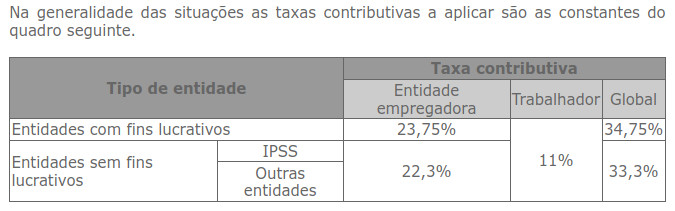
\includegraphics[width=.6\textwidth,left]{./image/SGS/Contribuicoes_1.jpg}
	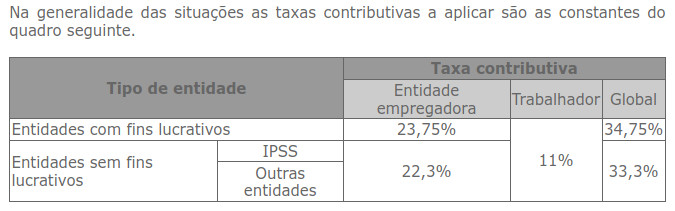
\includegraphics[scale=.5]{./image/SGS/Contribuicoes_1.jpg}
	\caption{Contribuições para SGS}
\end{figure}
\textbf{Exemplo:}
\newline
Vencimento de 1000Eur será descontado 11\% para a Segurança Social, ficando com $1000\times (1-0,11)=890Eur$ e a empresa desconta para o exemplo de 23,75\%, $1000\times 0,2375=237,5Eur$, ao todo será descontado $110+237,5=347,5Eur$, ou seja, todos os messes um trabalhador que ganhe 1000Eur desconta para a Segurança Social direto e indiretamente \textbf{347,5Eur}.
\emptyline
Na realidade o vencimento neste exemplo do cidadão devia ser de \textbf{1237,5Eur}, ou seja, é prejudicado nos seus descontos na quantia de 237,5Eur [23,75\%] pois não são considerados como pessoais. \\
A circulação deste capital passa despercebido e usado pelo estado para seus gastos, sendo o cidadão sua fonte, sem nenhum proveito, a não ser que talvez as empresas depois recebem ajudas através desta receita.
\emptyline
Em Geral a receita laboral de um cidadão é quase três oitavos $23,75\%+11\%=34,75\%$ depois dos respetivos descontos [1000Eur \textit{vs} 347,5Eur].
\emptyline
Estas contas são feitas sem considerar qualquer subsidio de alimentação.
\emptyline
\textcolor{green}{\small [ link: \quad http://www.seg-social.pt/trabalhadores-por-conta-de-outrem ]}
\subsection{Trabalhadores Independentes}
%%%%%%%%%%%%%%%%%%%%%%%%%%%%%%%%%%%%%%%%%%%%%%%%%%%%%%%%%%%%%%%%%
\qquad Este tipo de contribuinte em princípio pode definir seus descontos numa dada margem, e é aliciante para as empresas pois não tem qualquer responsabilidade, este acarreta toda a responsabilidade de descontos e despesas, no entanto em princípio ira ganhar mais do que o trabalhador por conta de outrem, mas descontando muito menos e prejudicado a longo prazo devido a concorrência, a não ser que desconte a totalidade de $23,75\%+11\%=34,75\%$ e ainda obter um vencimento superior ao seu equivalente de trabalhador por conta de outrem.
Os exemplos são trabalhadores a recibos verdes, subcontratados e a trabalho temporário.
\subsection{Precariedade}
%%%%%%%%%%%%%%%%%%%%%%%%%%%%%%%%%%%%%%%%%%%%%%%%%%%%%%%%%%%%%%%%%
\qquad Nenhum cidadão devia aceitar qualquer trabalho que ganhe menos que \; $ \mbox{\Large $ \frac{635Eur}{0,65}\approx 977Eur $ } $ para se dizer que leva uma vida sustentável, pois o salário mínimo nacional é de 635Eur, e se ficar em \textit{lay off} ou \textit{desempregado}, como demonstrado:
\emptyline
\hspace*{.3cm} $635\times(1-0,11)\approx566Eur$,\hspace*{1cm} $635\times(0,3475)\approx220Eur$,\hspace*{1cm} $\frac{635\times14}{12}\times0,65 \approx 482Eur$,
\emptyline
estará a trabalhar gratuitamente, só ira receber \textbf{566Eur} com descontos de \textbf{220Eur}, ou seja um escravo do estado. No caso de \textit{lay-off ou desemprego} recebera apenas 482Eur.\\
Em princípio qualquer remuneração será deduzido por: $Vencimento \times (1-0,11) \times (1-0,23) - Combustivel\times 0,61 = Rendimento \, Liquido$, pois tudo também leva \textit{IVA} e a taxa de combustível.
\emptyline
\textbf{Exemplo} (\textit{indivíduo com salário mínimo nacional}) \; \textbf{:}
\emptyline
1. vencimento = 635Eur e 0Eur gasolina mensal \\
\hspace*{1cm} $635Eur \times (1-0,11) \times (1-0,23) - 0Eur \times 0,61 = 435Eur$ \\
2. vencimento = 635Eur e 80Eur gasolina mensal \\
\hspace*{1cm} $635Eur \times (1-0,11) \times (1-0,23) - 80Eur \times 0,61 = 386Eur$ \\
3. vencimento = 635Eur e 150Eur gasolina mensal \\
\hspace*{1cm} $635Eur \times (1-0,11) \times (1-0,23) - 150Eur \times 0,61 = 343Eur$,
\emptyline
mas ainda não acaba aqui a pintura negra, supondo agora que o cidadão não tem caro, ou seja, recebe limpos 435Eur, ainda vai ter que pagar taxa água e saneamento (mínimo 11,3Eur) e taxa de luz (mínimo 8Eur). Fica com 415,7Eur, para piorar vamos supor que tem habitação e têm que pagar IMI (mínimo 11Eur/mês).
Se este exemplo tiver um empréstimo de habitação e ou um veiculo chegamos a conclusão que não pode se alimentar, o que será muito bom para a dieta, e doenças.
\emptyline
Concluindo que no estado presente de trabalho só é benéfico se pertencermos aos membros de órgãos estatuários ou político, pois não tem encargos do estado e aufere de regalias e vencimentos mínimo de cinco vezes e até dez vezes superior ao salário mínimo nacional, também existindo casos excecionais de vinte e para cima a mais o salário mínimo nacional. Sendo que esta profissão existe apenas por tráfico de influências e não igualdade ou equidade, muito menos competência, como demonstrado com esta pandemia na qual suas soluções para os problemas são solidariedade.
\subsection{Mudança}
%%%%%%%%%%%%%%%%%%%%%%%%%%%%%%%%%%%%%%%%%%%%%%%%%%%%%%%%%%%%%%%%%
\qquad Já é conhecido que em \textsf{2025}, 75\% da classe trabalhadora vai pertencer a geração \textbf{Y}, e o quadro do futuro de trabalho esta cada vez mais centrado a volta do desenvolvimento tecnológico, as sociedades vão ter que acompanhar o ritmo de crescimento, e a União Europeia e seus membros reconhecem esta tendência e a necessidade de formação e treino destas competências nos trabalhadores Europeus, sendo o projeto \textit{industria 4.0} uma destas ferramentas.
\begin{figure}[H]
	\centering
	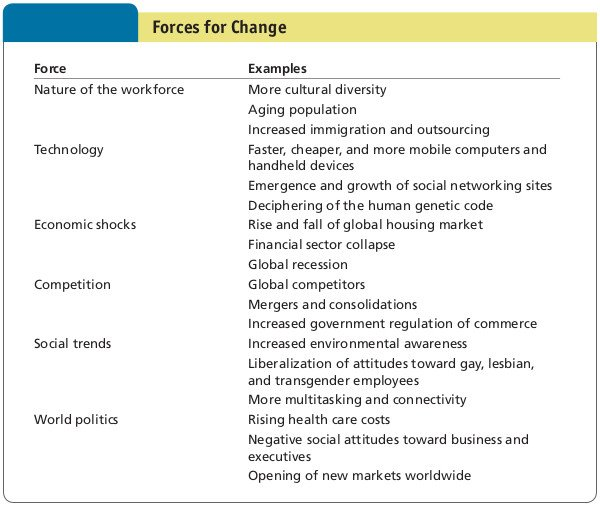
\includegraphics[scale=0.52]{./image/Change/Forces_for_Change.jpg}
	\caption{Forças para a Mudança \cite{book-7}}
\end{figure}
Empresas de todo tipo e dimensão estão a ser enfrentados com a questão de como podem assegurar o fornecimento de líderes com as competências, habilidades e visão estratégica adequadas para obter o sucesso. Ignorando a velha mentalidade de que certos indivíduos nascem para liderar, muitas empresas acreditam que a liderança pode ser desenvolvida numa forma pro-ativa e de forma sistemática. \cite{book-6}
\emptyline
A liderança assume um papel importante na mudança de cultura dentro das organizações e requer estar sempre em constante adaptação ao seu meio ambiente. Como sugere a liderança \textit{VUCA}, que representa Volatilidade, incerteza (uncertainty), complexidade e ambiguidade. Volatile porque não é estático esta e em constante mudança, incerteza na previsão do futuro, complexo com sistemas cada vez mais sofisticados que requer competências adequadas e ambíguo com problemas difícil de identificar, pouca informação de alternativas, sem se saber as consequências.
\begin{figure}[H]
	\centering
	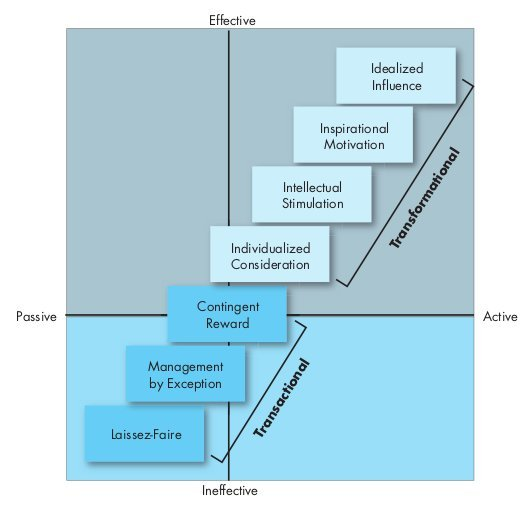
\includegraphics[scale=0.52]{./image/Leadership/Leadership_Models.jpg}
	\caption{Modelos da Liderança \cite{book-2}}
\end{figure}
Este trabalho esta focado no futuro do trabalho, gestão de carreira e marketing pessoal, no entanto abordar as matérias da gestão de mudança, a planeada (Modelo Kurt Lewin) e a emergente, os tipos de lideres, seus estilos e abordagens, também os modelos criados (Modelo Blake \& Mouton, Hersey \& Blanchard) são ferramentas úteis para nos orientar nos nossos comportamentos em diferentes contextos e determinar as atitudes a tomar com o nosso grupo ou equipa de forma a poder alcançar os objetivos e uma visão, ou seja garantir a sobrevivência e prosperidade da organização.
\begin{figure}[H]
	\centering
	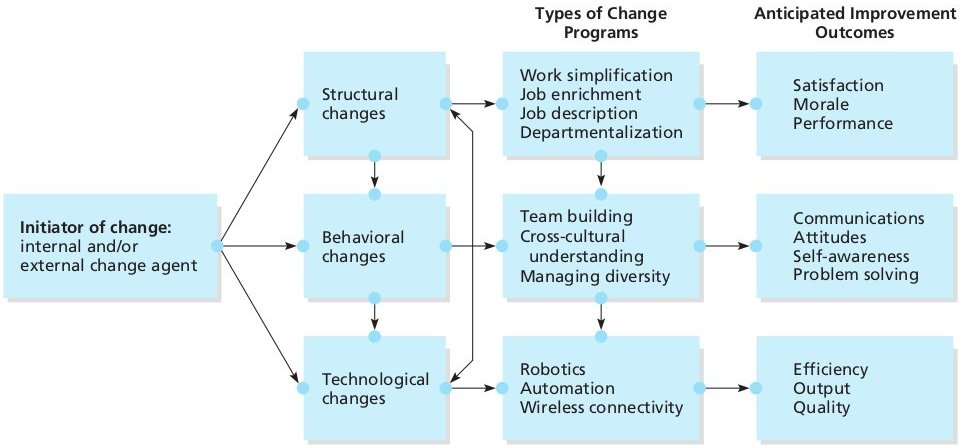
\includegraphics[scale=0.52]{./image/Change/Three_Change_Approaches.jpg}
	\caption{Três formas de mudar \cite{book-6}}
\end{figure}
 % Introduction
\section{Revisão da Literatura}
\qquad A disciplina \textcolor{blue}{Comportamento Organizacional} é uma ciência aplicada ao comportamento que é retirada de contribuições de disciplinas que estudam o comportamento, especificamente da psicologia e psicologia social, sociologia e antropologia.
As contribuições da psicologia são concentrada no individuo ou analise a nível micro, enquanto as outras disciplinas contribuíram para perceber a nível macro conceitos como procedimentos de grupo e organização.\cite{book_2}
\emptyline
Quadro das Contribuições para o estudo desta disciplina:
\begin{figure}[H]
\centering
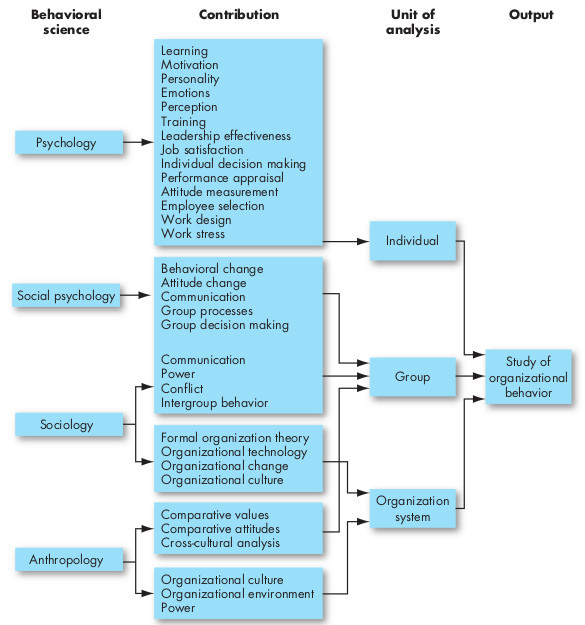
\includegraphics[scale=0.52]{./image/OB/OB_contributions.jpg}
\caption{Contribuições para OB \cite{book_2}}
\end{figure}
Este relatório esta focado no estudo da \textcolor{blue}{\textbf{Cultura Organizacional}}, portanto vou começar por definir o que é uma organização e seus objetivos.
\emptyline
%%%%%%%%%%%%%%%%%%%%%%%%%%%%%
Uma organização é um grupo estruturado de pessoas, um grupo onde cada pessoa é responsável por tarefas bem definidas e onde existe um sistema de articulação entre elas, que desenvolve um conjunto de atividades visando a definição e prossecução de objetivos comuns (de forma continuada no tempo). O objetivo das organizações é para criar valor para os seus clientes/utentes, para os detentores do seu capital, para os seus colaboradores, para os seus fornecedores e para a sociedade em geral.\cite{book_10}
%%%%%%%%%%%%%%%%%%%%%%%%%%%%%%%%%%%%%%%%%%%%%%%%%%%%%%%%%%%%%%%%%%%%%%%%%%%%%%%%%%%%%%%%%%%%%%%%%%%%%%%%%%%%%%%
\newpage
Todas as organizações estão inseridas num contexto Cultural que pertence a um País ou Região e pelo modelo criado por \textit{Geer Hofstede}, Portugal tem esta distribuição nas suas dimensões:
\begin{figure}[H]
\begin{minipage}{0.3\textwidth}
\flushleft
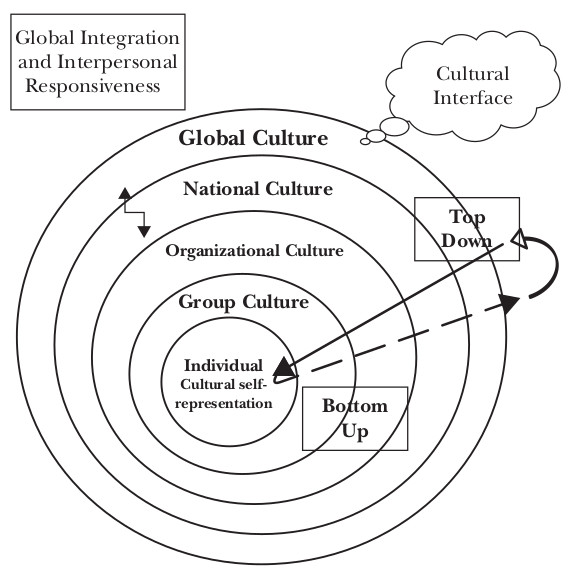
\includegraphics[scale=0.30]{./image/OB/OB_MUltilevelmodelCulture.jpg}
\end{minipage}
\hspace{.3cm}
\begin{minipage}{0.4\textwidth}
\flushleft
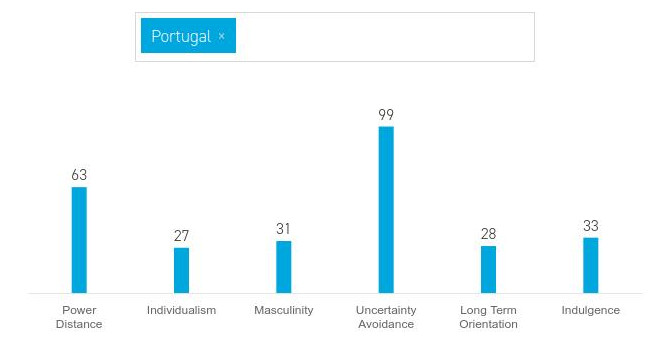
\includegraphics[scale=0.45]{./image/OB/Hofstede_pt.jpg}
\end{minipage}
\caption{Modelo de Multi-níveis \cite{book_11} da cultura e Modelo Hofstede, Portugal}
\end{figure}
Website:\\
\textit{\textcolor{green}{https://hi.hofstede-insights.com/national-culture}}
\emptyline
%%%%%%%%%%%%%%%%%%%%%%%%%%%%
Ambos a Cultura da Organização e o Comportamento da Liderança foram identificados como determinantes criticos para a eficácia da organização, que se deve adaptar ao contexto transacional e externo à organização. A Cultura Organizacional é um conjunto de valores, crenças e suposições partilhadas pelos membros de uma organização que a distingue das outras organizações, por exemplo, rituais e cerimonias, a historia da organização, sua estrutura e seus princípios.\cite{book_9}
\emptyline
%%%%%%%%%%%%%%%%%%%%%%%%%%%%%
A forma das organizações se identificarem e destacarem a sua cultura no mercado é expondo a sua \textcolor{blue}{Missão}, \textcolor{blue}{Visão} e seus \textcolor{blue}{Valores}.
\emptyline
%%%%%%%%%%%%%%%%%%%%%%%%%%%%%
A \textcolor{blue}{missão} é os objetivos na qual a organização pretende atingir, a \textcolor{blue}{visão} aonde pretendem chegar (futuro) e seus \textcolor{blue}{valores}, que são suas crenças e princípios na qual defendem, e mantêm a organização unida. Como vimos anteriormente pelo estudo de \textit{Geer Hofsteed} os valores são dependente das culturas.
\emptyline
%%%%%%%%%%%%%%%%%%%%%%%%%%%%%%
As Organizações podem ter diferentes características, e o \textcolor{blue}{\textbf{Modelo de Ogbonna \& Harris}}, carateriza a cultura das organizações em \textcolor{orange}{quatro} tipos, que pode ser análoga a outros modelos tais como o de \textbf{Handy} e \textbf{Cameron \& Quin}.
\begin{figure}[H]
\flushleft
\captionsetup{justification=raggedright,singlelinecheck=false}
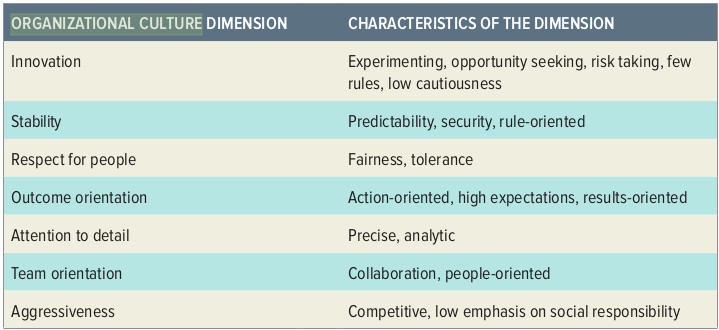
\includegraphics[scale=0.4]{./image/OB/OC_Dimensions.jpg}
\caption{Dimensões da Cultura Organizacional \cite{book_4}}
\end{figure}
A cultura de uma organização pode ser descrita como a perceção em que todos seus membros tem em comum acerca da organização, normalmente a maioria de grandes organizações podem ter uma cultura dominante com varias subculturas, sua cultura dominante reflect seus valores de raiz, e subculturas podem ter os valores de raiz mais alguns outros valores únicos dos seus membros de um dado departamento. \\
A cultura organizacional dominante pode ser medida em termos da quantidade em que seus membros estão alinhados com os valores de raiz. \\
As organizações devem criar uma cultura organizacional em que proporciona um \textcolor{blue}{clima} favorável para seus membros de forma a poderem ter um desempenho positivo, caso contrario pode ter o efeito contrario. A cultura organizacional é criada pelos fundadores da organização, com a responsabilidade de a sustentar e cuidar, mantendo seus valores éticos e de moralidade intactos para ter uma \textcolor{blue}{cultura positiva}. O papel da \textcolor{blue}{motivação} tem uma influencia importante na sua manutenção, deve promover a recompensa e delegação de poder.\cite{book_4} \cite{book_2}
%%%%%%%%%%%%%%%%%%%%%%%%%%%%%%%%%%%%%%%%%%%%%%%%%%%%%%%%%%%%%%%%%%%%%%%%%%%%%%%%%
 % Revisão da Literatura
\section{Organização}
\qquad A Empresa S.Roque ou ROQ
\emptyline
Localizada no coração do Vale do Ave, a S.Roque - Máquinas e Tecnologia Laser S.A., labora em instalações próprias com uma área coberta de aproximadamente 25.000 $m^{2}$. A empresa orgulha-se de ser hoje uma experiente e bem-sucedida PME, tendo sido distinguida pelo IAPMEI como PME Líder e de Excelência pelo quarto ano consecutivo.
\emptyline
Líder nacional no seu campo de atividade – fabrico de máquinas e equipamentos para as indústrias de estamparia têxtil e embalagem - emprega atualmente mais de 350 funcionários distribuídos pelos seus diferentes departamentos.
\emptyline
Com instalações funcionais e com profissionais qualificados e experientes, a S.Roque dispõe das mais avançadas ferramentas e tecnologias na área da metalomecânica, do design e da elaboração de produto. Os equipamentos fabricados são de conceção própria, desenhados por um departamento técnico altamente especializado para corresponder aos desígnios de projeto e com o objetivo de satisfazer qualitativamente as solicitações do cliente mais exigente.
\emptyline
Hoje, após a conquista e solidificação incontestável da liderança do mercado português, tornando-se num dos líderes mundiais na área da estamparia e da embalagem, a S.Roque produz e comercializa um extenso catálogo com diferentes produtos e trabalha com clientes/parceiros um pouco em todo o mundo: Espanha, França, Itália, Inglaterra, Alemanha, Holanda, Suécia, Romênia, África do Sul, Marrocos, Tunísia, Angola, Turquia, Kuwait, Índia, China, Vietnam, Malásia, Camboja, Rússia, Bulgária, Brasil, Argentina, Peru, Colômbia, Honduras, El Salvador e E.U.A.
\begin{figure}[ht]
\begin{center}
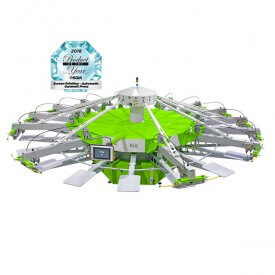
\includegraphics[scale=0.5]{./image/ROQ/maquinas/ECO-P18_600x600-2-275x275.jpg}
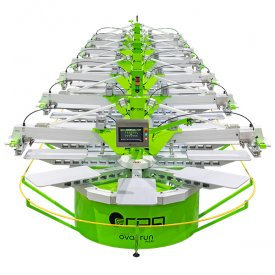
\includegraphics[scale=0.5]{./image/ROQ/maquinas/EVO-600x600-275x275.jpg}
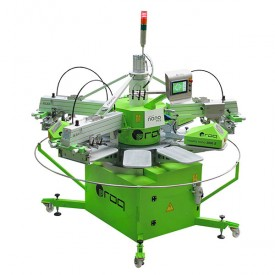
\includegraphics[scale=0.5]{./image/ROQ/maquinas/nanop10-275x275.jpg}
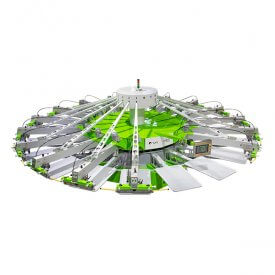
\includegraphics[scale=0.5]{./image/ROQ/maquinas/NEXTP18-600x6001-275x275.jpg}
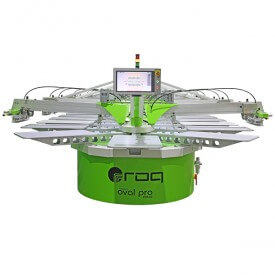
\includegraphics[scale=0.5]{./image/ROQ/maquinas/PRO-600x600-275x275.jpg}
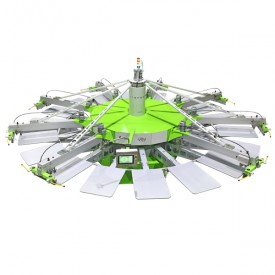
\includegraphics[scale=0.5]{./image/ROQ/maquinas/You-600x600-275x275.jpg}
\end{center}
\caption{Produtos Principais}
\end{figure}
%%%%%%%%%%%%%%%%%%%%%%%%%%%%%%%%%%%%%%%%%%%%%%%%%%%%%%%%%%%%%%%%%%%%%%%%%%%%%%%%%
\newpage
A S.Roque dedica-se à construção e comercialização de máquinas de estamparia têxtil há mais de 30 anos. Embora a sua génese esteja ligada à manutenção destes equipamentos, rapidamente foi identificada a oportunidade de construir de raiz este tipo de máquina. Os têxteis estavam em alta no Vale do Ave, e a S.Roque aproveitou para criar um produto de qualidade para uma clientela extremamente exigente. A empresa não se contentou em servir apenas o seu nicho de mercado, desde muito cedo que procurou a internacionalização. Numa primeira fase e por motivos geográficos criou parecerias europeias, numa segunda fase e por questões culturais dedicou-se ao Brasil e América do Sul. Neste milénio tornou-se numa marca global de referência na área onde atua. Todo e qualquer mercado está ao nosso alcance.\\
Hoje mais do que nunca não chega ter o melhor produto do mercado, é também necessário apresentar um serviço excelente e acessível em qualquer ponto do globo. A S.Roque orgulha-se de procurar a excelência em tudo em que se envolve com especial destaque para a procura de soluções.
\emptyline
Em 2015 a marca S.Roque transformou-se em ROQ. Atendendo às necessidades do século XXI reconhecemos a necessidade de criar uma marca verdadeiramente global que consiga de uma forma eficaz transmitir mais de 30 anos de história, inovação, internacionalização e conhecimento.
%%%%%%%%%%%%%%%%%%%%%%%%%%%%%%%%%%%%%%%%%%%%%%%%%%%%%%%%%%%%%%%%%%%%%%%%%%%%%%%%%
 % Organização
\section{Cultura Organizacional}
\qquad Os fundadores da organização têm um grande impacto no processo de formação da cultura organizacional através da imposição das suas crenças e suposições no grupo. A adoção das crenças, valores e suposições que formam a cultura da organização é depois reforçada pelos vários comportamentos primários dos lideres.\emptyline
%%%%%%%%%%%%%%%%%%%%%%%%%%
Planeamento Estratégico:
%%%%%%%%%%%%%%%%%%%%%%%%%%
\subsection{Missão}
A S.Roque tem como missão a constante inovação e criação de produtos de excelência na área da estamparia têxtil à peça. Para tal, aposta em múltiplos vetores complementares: tecnologia, qualidade e recursos humanos especializados. Estimula de forma persistente a sua veia empreendedora e internacional, promovendo para isso o contínuo aperfeiçoamento do seu serviço, em qualquer parte do mundo, mantendo-se fiel aos princípios éticos e de sustentabilidade.
%%%%%%%%%%%%%%%%%%%%%%%%%
\subsection{Visão}
Trilhar um percurso sustentável de inovação, de expansão internacional, de excelência em todas as soluções que lançamos para o mercado, de qualidade absoluta, para nos mantermos como líder na nossa área de negócio.
%%%%%%%%%%%%%%%%%%%%%%%%%%
\subsection{Valores}
\begin{itemize}
\setlength\itemsep{-0.3em}
\item Ação dentro dos princípios morais e éticos da empresa para com os seus \textit{stakeholders}.
\item Atuação sempre no interesse dos nossos parceiros de forma a promover a sua satisfação e fidelização.
\item Excelência conseguida através de trabalho de equipa, competência e responsabilidade.
\item Qualidade absoluta.
\item Inovação promovida pelo ADN empreendedor da S. Roque.
\item Sustentabilidade ambiental e segurança.
\end{itemize}\par
%%%%%%%%%%%%%%%%%%%%%%%%%%
Além da sua definição estratégica da cultura organizacional pode se fazer objetivos pelo método \textcolor{blue}{\textbf{SMART}}, para ajudar a definir a sua missão.
%%%%%%%%%%%%%%%%%%%%%%%%%%%%%%%%%%%%%%%%%%%%%%%%%%%%%%%%%%%%%%%%%%%%%%%%%%%%%%%%%
\subsection{Analise SWOT:}
A analise \textbf{SWOT} consiste em ver a organização em dois aspetos do ambiente onde estão inseridos, o interno e externo, e duas vertentes na qual terá influencia positiva ou negativa. O ambiente externo também tem duas vertentes que consiste no ambiente transacional e contextual com influencia \textcolor{blue}{PEST}, isto é, política, económica, social e tecnológico. Uma ferramenta muito útil para auxiliar na planificação.
\begin{itemize}
\setlength\itemsep{-0.5em}
\item \textcolor{purple}{I}nterno
\begin{itemize}
\setlength\itemsep{-0.3em}
\item \textcolor{orange}{S}trength (forças)\\
- Tem liderança no mercado interno, e reconhecimento internacional\\
- As maquinas são proprietárias\\
- Tem um mercado internacional\\
- Mão de obra qualificada é barata\\
- Tem um controlo de qualidade\\
- Dá suporte ao cliente\\
- Oportunidade de entrar noutros mercados
\item \textcolor{orange}{W}eakness (fraquezas)\\
- Mercado saturado internamente\\
- Localidade de produção isolado\\
- Dificuldade em obter mão de obra\\
- Portugal é reconhecido por ter má gestão\\
- Dificuldade em obter mão de obra qualificada
\end{itemize}
\item \textcolor{purple}{E}xterno
\begin{itemize}
\setlength\itemsep{-0.3em}
\item \textcolor{orange}{O}pportunity (oportunidades)\\
- Fácil acesso ao credito\\
- Inserido num país europeu com mão de obra barata\\
- Inserido numa sociedade femininista\\
- Ajudas do estado para o desenvolvimento (ex: programa 2020)\\
- Tecnologia mais recentes ao dispor
\item \textcolor{orange}{T}hreats (ameaças)\\
- A competir com mercado internacional mais forte\\
- Areá têxtil sob ameaça\\
- Sociedade que evita a incerteza
\end{itemize}
\end{itemize}
%%%%%%%%%%%%%%%%%%%%%%%%%%%%%%%%%%%%%%%%%%%%%%%%%%%%%%%%%%%%%%%%%%%%%%%%%%%%%%%%%
 % Cultura Organizacional
\section{Estudo da Cultura Organizacional segundo o Modelo Ogbonna \& Harris}
\qquad O Modelo Ogbonna \& Harris estuda a relação entre as variáveis de Estilos de liderança, Cultura organizacional e Performance organizacional. Este modelo foi derivado de um estudo empírico na Inglaterra através de os procedimentos científicos e estatísticos sobre a analise dos dados obtidos por questionários às empresas envolvidas.
%%%%%%%%%%%%%%%%%%%%%%%%%%%%%%%%%%%%%%%%%%%%%%%%%%%%%%%%%%%%%%%%%%%%%%%%%%%%%%%%%
\subsection{Modelo Ogbonna \& Harris}
\quad {\bf As variáveis  descritas de seguida, são as que foram consideradas no estudo.}
\emptyline
\begin{minipage}[t]{.31\linewidth}
\quad Estilos de Liderança:
\begin{itemize}
\setlength\itemsep{-0.3em}
\item Participativo
\item Orientado as pessoas\\
(Liderança de suporte)
\item Orientado as tarefas\\
(Liderança Instrumental\\ ou Diretiva\\ ou Transacional)
\end{itemize}
\end{minipage}
\begin{minipage}[t]{.31\linewidth}
\quad Tipos de Cultura:
\begin{itemize}
\setlength\itemsep{-0.3em}
\item Inovadora
\item Competitiva
\item Burocrática
\item Comunitária
\end{itemize}
\end{minipage}
\begin{minipage}[t]{.31\linewidth}
\quad Medição do Sucesso:
\begin{itemize}
\setlength\itemsep{-0.3em}
\item Satisfação dos Clientes
\item Taxa crescimento vendas
\item Cotação no mercado
\item Vantagens Competitivas
\item Volume de vendas
\end{itemize}
\end{minipage}
\minipagespace{.5cm}
Os resultados obtidos na determinação do estilo de liderança e tipo de cultura organizacional das empresas estudadas, e o modelo que foi criado são apresentados de seguida:
\begin{figure}[H]
\centering
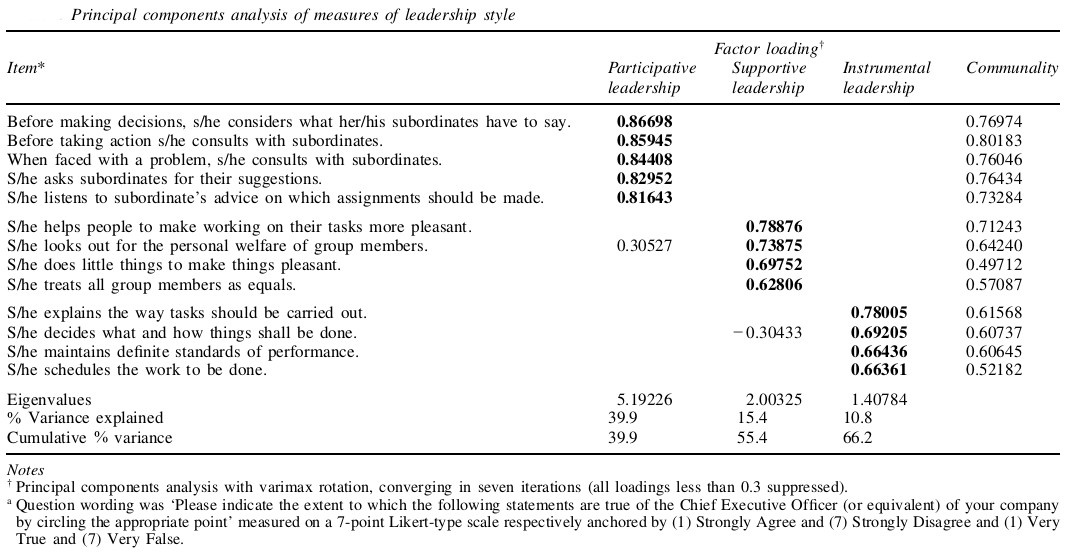
\includegraphics[scale=.4]{./image/OB/Leadership.jpg}\\
\caption{Inquérito do Estilos de Liderança \cite{article_1}}
\end{figure}\par
%%%%%%%%%%%%%%%%%%%%%%%%%%%%%%%%%%%%%%%%%%%%%%%%%%%%%%%%%%%%%%%%%%%%%%%%%%%%%%%%%
A tabela acima é o inquérito com os resultados das 322 companhias que serviram de amostras. Os resultados depois foram tratados por um método estatístico de forma a obter o modelo. Os estilos de liderança depois são determinado através do peso das questões que caraterizam cada uma.
%%%%%%%%%%%%%%%%%%%%
\begin{figure}[H]
\centering
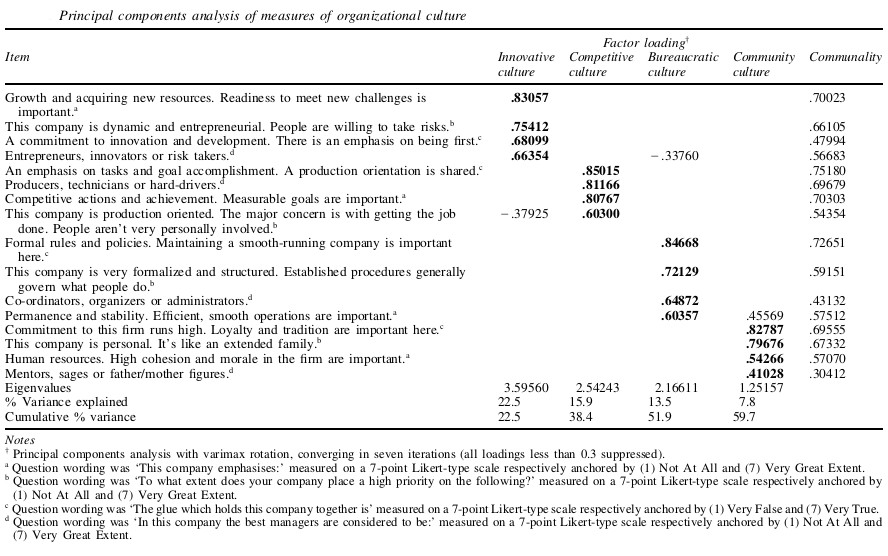
\includegraphics[scale=.5]{./image/OB/Culture.jpg}\\
\caption{Inquérito do tipo de Cultura Organizacional \cite{article_1}}
\end{figure}\par
%%%%%%%%%%%%%%%%%%%%
A tabela acima, demonstra as questões e os tipos de cultura que representam, em conjunto com a tabela do estilo de liderança e o tratamento dos dados Ogbonna \& Harris obterem o seu modelo.
%%%%%%%%%%%%%%%%%%%%
\begin{figure}[H]
\centering
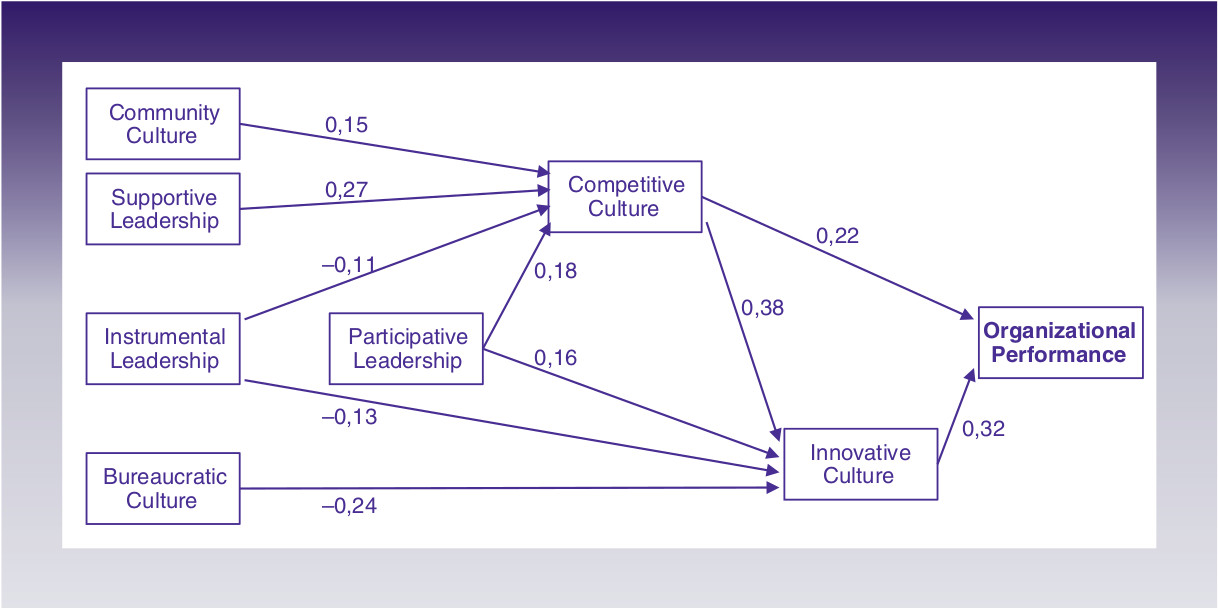
\includegraphics[scale=.35]{./image/OB/Ogbonna_Harris.jpg}\\
\caption{Modelo Ogbonna \& Harris \cite{article_1}}
\label{Modelo}
\end{figure}
Neste estudo foi observado que a relação entre o estilo de liderança e o sucesso não era tão bem percebido como a relação entre a de cultura organizacional e o sucesso. Descobriram que a cultura organizacional servia de mediador entre o estilo de liderança e o sucesso. O estilo de liderança não tinha influencia direta no seu sucesso mas indiretamente. Descobriram também que organizações com o tipo de cultura inovadora e competitiva eram mais bem sucedidas do que as companhias com cultura organizacional burocráticas ou comunitárias. A cultura inovadora e competitiva era mais focada para o exterior (posicionamento e resposta), e a cultura burocrática e comunitária para o interior (integração, coesão, uniformidade). As companhias com culturas burocráticas e comunitárias demonstravam uma relação insignificante e indireta entre cultura organizacional e sucesso, no entanto para as culturas inovadoras e competitivas existia uma forte e positiva relação. Enquanto, a cultura inovadora e competitiva preenchia quase 25 \% da variância na performance das organizações (sucesso), também se observou que apenas o tipo de liderança participativa e orientada às pessoas tinham uma correlação positiva com as culturas inovadoras e competitivas.
\emptyline
Concluindo que, as organizações com culturas inovadoras e competitivas, tendo um estilo de liderança orientada às pessoas e participativa seriam mais promissoras para melhorar o desempenho da organização e que devem focar-se em \textcolor{blue}{mudar} para uma cultura orientada para o exterior. \cite{article_1}
%%%%%%%%%%%%%%%%%%%%%%%%%%%%%%%%%%%%%%%%%%%%%%%%%%%%%%%%%%%%%%%%%%%%%%%%%%%%%%%%%
\subsection{Modelo Aplicado a S.Roque}
O Inquérito (\textit{igual figura 6}) abaixo é usado para medir os componentes principais para determinar a Cultura Organizacional.
\begin{table}[H]
\begin{adjustbox}{max width=\textwidth}
\begin{tabular}{ |c|l|c| }
\hline
\rowcolor[gray]{0.5}
Nº & Inquérito & \makecell[l]{Resp \\ 1 \; - \; 7} \\
\hline
1. & \makecell[l]{A organização preocupa-se com o crescimento e a aquisição de novos recursos, \\ e procura responder a novos desafios.} & \\
\hline
2. & \makecell[l]{A organização é dinâmica e empreendedora. \\ As pessoas estão dispostas a correr riscos.} & \\
\hline
3. & \makecell[l]{Existe um elevado empenho na inovação e no desenvolvimento. \\ Procuramos ser os primeiros.} & \\
\hline
4. & \makecell[l]{Consideram-se os melhores gestores os que são empreendedores, \\ Inovadores e tomadores de riscos.} & \\
\hline
5. & Existe uma elevada ênfase nas tarefas e no alcance de objetivos. & \\
\hline
6. & Considera-se que os melhores gestores são produtores e técnicos. & \\
\hline
7. & \makecell[l]{A organização valoriza as ações competitivas, \\ o sucesso e o alcance de objetivos mensuráveis.} & \\
\hline
8. & \makecell[l]{A organização é orientada para a produção. \\ Uma das maiores preocupações é fazer o que tem que ser feito. \\ Os empregados não estão muito envolvidos do ponto de vista pessoal.} & \\
\hline
9. & A organização valoriza muito as regras e as políticas formais. & \\
\hline
10. & \makecell[l]{A organização é muito formalizada e estruturada. \\ Os procedimentos estabelecidos orientam o que as pessoas devem fazer.} & \\
\hline
11. & Os melhores gestores são considerados os que são coordenadores ou organizadores. & \\
\hline
12. & Na organização valoriza-se a permanência, a estabilidade e a eficiência. & \\
\hline
13. & Valoriza-se muito a lealdade, a tradição e o empenhamento na organização. & \\
\hline
14. & A organização é uma espécie de grande família. & \\
\hline
15. & Valoriza-se muito a coesão e os recursos humanos. & \\
\hline
16. & \makecell[l]{Considera-se que os melhores gestores são os que atuam como mentores, \\ sábios ou figuras paternais/maternais.} & \\
\hline
\end{tabular}
\end{adjustbox}
\end{table}
{\tiny 1- A afirmação não se aplica rigorosamente nada à minha organização, 2- Não se aplica, 3- Aplica-se muito pouco, 4- Aplica-se alguma coisa,\\ 5- Aplica-se bastante, 6- Aplica-se muito, 7- A afirmação aplica-se completamente à minha organização
}
%%%%%%%%%%%%%%%%%%%%%%%%%%%%%%%%%%%%%%%%%%%%%%%%%%%%%%%%%%%%%%%%%%%%%%%%%%%%%%%%%
\begin{table}[H]
{\small
\begin{tabular}{|l|c|c|}
\hline
                                                                                                    & Média do Inquerito & \begin{tabular}[c]{@{}l@{}}Ogbonna \& Harris\\ (2000)\end{tabular} \\ \hline
\cellcolor[HTML]{C0C0C0}\begin{tabular}[c]{@{}l@{}}Cultura de inovação\\ {[}1-4{]}\end{tabular}     & 5,4 & 4,6 \cellcolor[HTML]{EFEFEF}                                           \\ \hline
\cellcolor[HTML]{C0C0C0}\begin{tabular}[c]{@{}l@{}}Cultura de Competição\\ {[}5-8{]}\end{tabular}   & 5,3 & 4,2 \cellcolor[HTML]{EFEFEF}                                           \\ \hline
\cellcolor[HTML]{C0C0C0}\begin{tabular}[c]{@{}l@{}}Cultura Burocrática\\ {[}9-12{]}\end{tabular}    & 4,7  & 4,3 \cellcolor[HTML]{EFEFEF}                                           \\ \hline
\cellcolor[HTML]{C0C0C0}\begin{tabular}[c]{@{}l@{}}Cultura de Comunidade\\ {[}13-16{]}\end{tabular} & 5  & 4,6 \cellcolor[HTML]{EFEFEF}                                           \\ \hline
\end{tabular}
}
\end{table}
%%%%%%%%%%%%%%%%%%%%%%%%
{\footnotesize
\textbf{Contribuições para o Inquérito:}\\
\textbf{-} \; \textcolor{green}{Paulo Campos} ; \quad \textcolor{green}{Daniel Carvalho} ; \quad \textcolor{green}{Bruno Pereira} ; \quad \textcolor{green}{Sérgio Santos}
}
%%%%%%%%%%%%%%%%%%%%%%%%%%%%%%%%%%%%%%%%%%%%%%%%%%%%%%%%%%%%%%%%%%%%%%%%%%%%%%%%%
 % Estudo da Cultura Organizacional segundo o Modelo Ogbonna & Harris
\section{Conclusões}
\qquad Pelo resultado do inquérito feito pode-se dizer que a S.Roque aponta para uma cultura predominantemente \textcolor{blue}{inovadora}, com um grau elevado de incerteza devido ter muito poucas amostras. Com este inquérito, deu para perceber que cada individuo tem uma perceção diferente da organização, o que leva a crer que a S.Roque não tem uma cultura forte. O estilo de liderança é mais orientado ás tarefas, ou seja, uma liderança transacional ou instrumental.
\emptyline
%%%%%%%%%%%%%%%%%%%%%%%%%%%
A S.Roque tem orgulho em afirmar que é o primeiro no nosso mercado interno e destaca-se internacionalmente. O seu sucesso poderá ser medido recorrendo ao \textcolor{blue}{benchmarking} que o confirma. Também a nível de satisfação dos seus clientes não obtive nenhuma informação pelo método \textcolor{blue}{scorecard management}, e no seu site não tem indicações relacionadas. O \textcolor{blue}{Banco de Portugal} também é outra fonte onde é possível verificar o sucesso da organização quanto ao seu histórico de capital. O desempenho da organização pode no final ser demonstrado através da sua eficácia e eficiência.
\emptyline
As melhores práticas podem ser consultadas em fontes como a American National Standards Institute (ANSI) ou a Canadian Standards Association (CSA), ou internacional, tais como as normas ISO ou Institute of Electrical and Electronics Engineers (IEEE), e IEC.\\
%%%%%%%%%%%%%%%%%%%%%%%%%%
Na S.Roque como se trabalha com equipamentos elétricos e eletrónicos, tem que respeitar normas e diretivas em vigor de cada produto, tendo sempre em consideração a qualidade. Tem que ter indivíduos com formação especifica, com autonomia no seu trabalho. Os produtos só são considerados prontos para o mercado depois de montados e testados nas suas instalações, assim têm uma boa base de garantia, evitando erros e reclamações.\\
Os colaboradores tem um ambiente sem pressões e com tarefas pré-determinadas, o único ponto desfavorável talvez é de ser trabalho monótono, tendo que se criar tarefas rotativas, que nem sempre é possível por ter diferentes especialidades.
\emptyline
%%%%%%%%%%%%%%%%%%%%%%%%%%%
O estudo Ogbonna \& Harris também nos demonstrou que um líder participativo, isto é, o que permite que os seus subordinados possam influenciar nas suas decisões pelas suas opiniões e contribuições e o líder de suporte que está focado ao bem estar dos colaboradores, tendo uma atitude amigável e simpática são mais prósperos a obter resultados positivos.\\
O líder instrumental tendo um desempenho negativo, pois esta orientado em criar expectativas, estabelecer procedimentos e atribuir tarefas.\\
A S.Roque aqui pode tirar partido destas observações, não retirando a importância do papel da comunicação, a motivação e resolução de problemas.
A satisfação dos colaboradores e perspectivas de desenvolverem, são fatores que contribuem positivamente. Como se sabe não vale a pena remar o barco se não se sabe o destino.
\emptyline
%%%%%%%%%%%%%%%%%%%%%%%%%%%
Neste relatório a matéria abordada é a \textcolor{blue}{Cultura Organizacional}, com varias indicações comprovadas e medidas, que deve servir de apoio às organizações, e foi demonstrado na sua elaboração. Esta disciplina é muito enriquecedora, existindo uma vasta informação literária com suporte bastante alargado na \textit{internet}, para os que quiserem desenvolver os temas abordados.
%%%%%%%%%%%%%%%%%%%%%%%%%%%%%%%%%%%%%%%%%%%%%%%%%%%%%%%%%%%%%%%%%%%%%%%%%%%%%%%%%
 % Conclusões

\bibliography{./bibliography/Bibliography}
\appendix
%\include{<location appendix>}
\newpage
\footnote{Apontamento}
\end{document}
%%%%%%%%%%%%%%%%%%%%%%%%%%%%%%%%%%%%%%%%%%%%%%%%%%%%%%%%%%%%%%%%%
%%%%%%%%%%%%%%%%%%%%%%%%%%%%%%%%%%%%%%%%%%%%%%%%%%%%%%%%%%%%%%%%%
%\selectbiblanguage{portuguese}
%\setbtxfallbacklanguage{english}
%%%%%%%%%%%%%%%%%%%%%%%%%%%%%%%%%%%%%%%%%%%%%%%%%%%%%%%%%%%%%%%%%%%%%%%%%%%%%%%%%
%%%%%%%%%%%%%%%%%%%%%%%%%%%%%%%%%%%%%%%%%%%%%%%%%%%%%%%%%%%%%%%%%%%%%%%%%%%%%%%%%
\begin{comment}
Usando o método Socrático podemos perguntar qual a melhor ou melhores culturas organizacional que se enquadra na nacional nos vários tipos de organizações existentes.\\
%%%%%%%%%%%%%%%%%%%%%%%%%%%%
Para criar uma cultura na organização deve-se definir uma missão, valores, visão e os objetivos.\\
%%%%%%%%%%%%%%%%%%%%%%%%%%%%
Durante muito tempo tem havido estudos para descobrir a formula mágica que leva as organizações a ter sucesso, existe muitas abordagens com diferentes perspectivas, algumas convergem e outras divergem, e assim foram criados novos conceitos de forma a encapsular estilos e tipos de forma a poder se identificar quais são os mais propícios a ter uma maior elevada taxa de sucesso, conceitos tais como comportamento organizacional, cultura organizacional, performance organizacional, etc.\\
%%%%%%%%%%%%%%%%%%%%%%%%%%%%%
GENDER:
Nearly half of the U.S. workforce is now made up of women, and women are a growing percentage of the workforce in most countries throughout the world. Organizations need to ensure that hiring and employment policies create equal access and opportunities to individuals, regardless of gender.
RACE:
The percentage of Hispanics, blacks, and Asians in the U.S. workforce continues to increase. Organizations need to ensure that policies provide equal access and opportunities, regardless of race.
NATIONAL ORIGIN:
A growing percentage of U.S. workers are immigrants or come from homes where English is not the primary language spoken. Because employers in the United States have the right to demand that English be spoken at the workplace during job-related activities, communication problems can occur when employees’ English language skills are weak.
AGE:
The U.S. workforce is aging, and recent polls indicate that an increasing percentage of employees expect to work past the traditional retirement age of 65. Organizations cannot discriminate on the basis of age and need to make accommodations for the needs of older workers.
DISABILITY:
Organizations need to ensure that jobs and workplaces are accessible to the mentally, physically, and health challenged.
DOMESTIC PARTNERS
An increasing number of gay and lesbian employees, as well as employees with live-in partners of the opposite sex, are demanding the same rights and benefits for their partners that organizations have provided for traditional married couples.
RELIGION:
Organizations need to be sensitive to the customs, rituals, and holidays, as well as the appearance and attire, of individuals of non-Christian faiths such as Judaism, Islam, Hinduism, Buddhism, and Sikhism, and ensure that these individuals suffer no adverse impact as a result of their appearance or practices.
Tipos de descriminação:
sexual, intimidação, insultos e coerção, exclusão, incivilidade.
A satisfação melhora o desempenho.\\
%%%%%%%%%%%%%%%%%%%%%%%%%
Nas empresas publicas, o estimulo é sentido em menor grau ou não existente, consoante o tipo e características concretas da organização.\\
%%%%%%%%%%%%%%%%%%%%%%%%%
Nas organizações sem fim lucrativos e/ou dependentes do estado, existe outro tipo de estimulo os interesses dos governantes, quando o estado é parceiro ou responsável pela organização, os interesses de grupos de pressão da sociedade, etc.\\
%%%%%%%%%%%%%%%%%%%%%%%%%
Nas organizações sem fins lucrativos os objetivos estão em permanente discusão e/ou a ser alterados, resultando uma maior indefinição sobre as atividades a desenvolver por responsáveis e por colaboradores.\\
%%%%%%%%%%%%%%%%%%%%%%%%%
Teoria de Geer Hofteed.\\
%%%%%%%%%%%%%%%%%%%%%%%%%%
Best practices can come from national, say the American National Standards Institute (ANSI) or the Canadian Standards Association (CSA), or international, say ISO or Institute of Electrical and Electronics Engineers (IEEE), standards organizations, professional associa-tions, or consulting firms.\\
%%%%%%%%%%%%%%%%%%%%%%%%%
Eliminar desperdício e resolução de problemas.\\
%%%%%%%%%%%%%%%%%%%%%%%%%
Confiança na liderança e operadores.\\
%%%%%%%%%%%%%%%%%%%%%%%%%
Leaders have long been viewed as a primary influence on the creation of organizational culture (e.g. Bennis and Nanus, 1985; Schein, 1983). According to Schein (1985), the “only thing of real importance that leaders do is to create and manage culture”\\
%%%%%%%%%%%%%%%%%%%%%%%%%
Constante mudança de adaptação ao meio ambiente.\\
%%%%%%%%%%%%%%%%%%%%%%%%%
acknowledge that even in US and European companies, success rates are
not spectacular regarding efforts to change vision, values, and culture or business systems
and processes (Beer and Nohria, 2000; Beer et al., 1990; Carr et al., 1996).\\
%%%%%%%%%%%%%%%%%%%%%%%%%
Característica de bons Objetivos\\
- Claros\\
- Concisos\\
- Calendarizados\\
- Atingíveis\\
%%%%%%%%%%%%%%%%%%%%%%%%%
Tipos de organizações\\
- Organização privadas com fins lucrativos\\
- Organização privadas sem fins lucrativos\\
- Organização publicas com fins lucrativos\\
- Organização publicas sem fins lucrativos\\
%%%%%%%%%%%%%%%%%%%%%%%%%
tipos de hierarquias\\
tipos de departamentalizações\\
organização por processo\\
%%%%%%%%%%%%%%%%%%%%%%%%%
A divisão do trabalho, permitiu a redução do tempo de aprendizagem, isto é, cada um tem as suas funções, aumentando a produtividade. Cada um executa uma parte das tarefas necessárias a fabricação.\\
%%%%%%%%%%%%%%%%%%%%%%%%%
Gestão:
\emptyline
\begin{minipage}{20cm}
\begin{minipage}{5cm}
Instrumentos
\begin{enumerate}
\item Planear
\item Organizar
\item Controlar\\ \\
\end{enumerate}
\end{minipage}
\begin{minipage}{5cm}
Funções
\begin{enumerate}
\item Liderança
\item Comunicação
\item Motivação
\item Tomada de decisão
\end{enumerate}
\end{minipage}
\end{minipage}
%%%%%%%%%%%%%%%%%%%%%%%%%
Cadeia de valor\\
-Atividades principais\\
-Atividades de suporte\\
%%%%%%%%%%%%%%%%%%%%%%%%%
Cadeia de valor da organização é a sequencia de atividades e fluxos de informação que uma organização e os seus fornecedores devem desenvolver para desenhar, produzir, oferecer, entregar e suportar os seus produtos, estas são as atividades principais.\\
%%%%%%%%%%%%%%%%%%%%%%%%%
As atividades de suporte são as que apoiam um bom desempenho na realização das actividades principais.\\
- atividade administrativa e financeira\\
- atividade da gestão do pessoal\\
- atividade jurídica\\
- planeamento, controlo e gestão\\
- gestão de sistemas e tecnologia\\
%%%%%%%%%%%%%%%%%%%%%%%%%%
A atividade de suporte não contribuem diretamente para a criação do valor.\\
%%%%%%%%%%%%%%%%%%%%%%%%%%
Atividades de suporte e principal.\\
funções da Gestão sã Instrumental, Comportamental e Estrutural.\\
%%%%%%%%%%%%%%%%%%%%%%%%%%
Cumprir os objetivos é ser eficaz.\\
%%%%%%%%%%%%%%%%%%%%%%%%%%%
Para gerir a produção (planear, organizar, dirigir e controlar), há que recolher um elevado volume de informação de controlo, sendo frequentemente necessário refazer o planeamento.\\
%%%%%%%%%%%%%%%%%%%%%%%%%%%
- Implementação por projeto\\
- Implementação por processo\\
- Implementação por células\\
- Implementação por cadeia ou em linha\\
- Implementação por produto\\
%%%%%%%%%%%%%%%%%%%%%%%%%%
Na implementação por célula de fabrico procura agrupar os produtos segundo a semelhança das suas rotinas operatórias.\\
Na implementação por processo, é possível cada serie (ou lote) ser processado integralmente num dado centro, antes de avançar para o centro onde irá sofrer a operação de transformação seguinte.\\
A análise ABC pode ser utilizada para averiguar quais as principais encomendas responsáveis pela sobrecarga de um dado centro de trabalho.\\
%%%%%%%%%%%%%%%%%%%%%%%%%%
Organizar é estipular quem faz o quê, atribui-se os recursos necessários para o fazer, criar um sistema de informação para verificar execução.\\
%%%%%%%%%%%%%%%%%%%%%%%%%%%
O que lhes chama a atenção e medem; suas reações a incidentes criticos, alocação de meios, papeis assumidos, e partilha de informação; recompensas e delegação de poder; recrutamento, seleção e promoção. As lideranças chave tem como responsabilidade de modificar a cultura de forma a estar atualizada com as mudanças exigidas.\\
%%%%%%%%%%%%%%%%%%%%%%%%%%%%
Aqui distingue-se dois tipos de lideres os transacionais e os de transformação. “culture affects leadership  as much as leadership affects culture”
%%%%%%%%%%%%%%%%%%%%%%%%%%%%
Planear é estabelecer os objetivos a atingir e o percurso de ações.\\
%%%%%%%%%%%%%%%%%%%%%%%%%%%%
A formulação, avaliação e seleção de estratégias e o desenvolvimento dos planos mais detalhados para as pôr em prática são feitos após a definição da missão e da análise do meio ambiente da organização.\\
%%%%%%%%%%%%%%%%%%%%%%%%%%%%
Ferramentas para avaliar o cumprimento dos objetivos\\
- benchmarking\\
- scorecard management\\
- Banco de Portugal\\
%%%%%%%%%%%%%%%%%%%%%%%%%%%%
Método de demonstrar o desempenho de uma organizações através da eficacia, eficiência e seu rendimento.\\
%%%%%%%%%%%%%%%%%%%%%%%%%%%%%
Eficacia avalia em que medida os objetivos estão alinhados com a necessidades sociais que ela se propõe a satisfazer, ou seja, em que medida os seus objetivos são a tal adequados.\\
%%%%%%%%%%%%%%%%%%%%%%%%%%%%%
Eficiência avalia a economia de recursos utilizados para realizar os seus objetivos, requer uma boa estruturação dos processos seguidos nas atividades, o que leva tempo e custa dinheiro.\\
%%%%%%%%%%%%%%%%%%%%%%%%%%%%%
Missão - SWOT Meio Ambiente (transacional e contextual(PEST)) - Objetivos - Implementação.\\
%%%%%%%%%%%%%%%%%%%%%%%%%%%%%
O sucesso das empresas está correlacionada positivamente com o seu planeamento.\\
%%%%%%%%%%%%%%%%%%%%%%%%%%%%%
Na análise do meio ambiente transacional, analisa-se o comportamento previsional das entidades com quem a organização interage.\\
%%%%%%%%%%%%%%%%%%%%%%%%%%%%%
Controlo.\\
O controlo pode ser encarado como um processo de aprendizagem.\\
O controlo deve servir, acima de tudo, para ajudar a garantir que os objetivos estabelecidos são atingidos.\\
Se a informação recolhida e os resultados apurados no processo de controlo não conduzem a ações de correção quando necessário, este será não só inútil, mas até prejudicial.\\
O recurso aos sistemas de informação permite, em geral, simplificar os procedimentos de controlo.\\
%%%%%%%%%%%%%%%%%%%%%%%%%%%%%%%
Controlar é os procedimentos de verificar sua execução, estar atento a imprevistos e pronto a correções recorrendo a re-organização e/ou novo planeamento, também pode-se optar por não fazer nada.\\
%%%%%%%%%%%%%%%%%%%%%%%%%%%%%%%%
Estilos de liderança:
\begin{itemize}
\item participative leadership\\
Is gauged by the extent to which leaders allow subordinates to influence decisions by requesting input and contribution.
\item supportive leadership\\
Focuses on the degree to which the behaviour of a leader can be viewed as sympathetic, amicable, and considerate of subordinate needs.
\item Instrumetal leadership\\
This measure of leadership style is akin to directive or transactional leadership and is designed to measure the extent to which leaders specify expectations, establish procedures, and allocate tasks.
\end{itemize}
Motivação teorias Moslow, Hersberg, Victor Vroom.\\
Se as condições e recompensas oferecidas aos funcionários não lhes permitirem satisfazerem algumas das suas necessidades, mais facilmente abandonam a equipa ou organização a que pertencem.\\
Motivação é o conjunto de fatores que provocam, canalizam e sustentam o comportamento das pessoas.\\
Um gestor interessado em atingir um bom desempenho estabelece objetivos atingíveis e bem defendidos.\\
Auto-confiança no desenvolvimento do trabalho pode diminuir a sua motivação.\\
Motivar é criar condições necessárias para que as pessoas se empenham na prossecução dos objetivos da organização.\\
O impacto da comunicação no desempenho da organização é muito elevado.\\
Os Gestores tem de ser coerentes e alinhados com o que transmitem de forma a criar uma estrutura de confiança.\\
Um líder de uma organização é aquele que detém capacidades de influenciar os colaboradores.\\
gestão das atividades é o exercício do poder de um gestor.\\
poder de premiar e punir é suficiente para gerir as atividades do dia a dia.\\
poder informacional.\\
Um sistema de avaliação do desempenho de uma empresa é uma valia porque é uma boa oportunidade para analisar o grau de cumprimento dos objetivos acordados.\\
A medida que as organizações se achatam, os gestores têm de aprender a permitir que os seus colaboradores tomem decisões e tenham informação sobre questões mais sensíveis.\\
Para um engenheiro é muito útil conhecer os aspectos essenciais da legislação laboral.\\
A gestão das pessoas é cada vez mais importante porque são as pessoas que têm o conhecimento e só as pessoas o podem partilhar e aplicar.\\
Numa organização, apoiar e compensar as pessoas é fundamental, mas também é indispensável falar com elas sobre os erros que cometem no sentido de serem corrigidas e evitadas no futuro.\\
Uma organização tem maior probabilidade de ter sucesso se gerir as pessoas de modo a que estas ao contribuírem para o sucesso da organização tenham também sucesso elas próprias.\\
A qualidade é a totalidade das características de um produto ou serviço, que determinam a sua aptidão para satisfazer determinadas necessidades.\\
Garantia da qualidade tem como objetivo primeiro, o controlo do processo, ou seja, a minimização ou mesmo eliminação dos erros na produção.\\
A garantia da qualidade concentra-se no controlo do processo produtivo e controlo do produto.\\
Os custos relacionados com a insatisfação dos clientes são considerados custos de não qualidade.\\
O diagrama de Pareto permite identificar rapidamente as causas vitais e as triviais de um dado problema.\\
As cartas de controlo destinam-se a detetar as variações resultantes da alteração, frequentemente de natureza aleatória e acidental, de algum dos parâmetros de processo de fabrico (ditas causas especiais).\\
As sete ferramentas clássicas da qualidade\\
- Fluxograma\\
- Registo e análise de dados\\
- Diagrama de causa - efeito (espinha de peixe 4M)\\
- Diagrama de Pareto\\
- Histogramas\\
- Diagramas de dispersão\\
- Cartas de Controlo\\
tipos de lideres\\
- Autocrático\\
- Participativo \\
- Democrático \\
- Deixa andar\\
estilo de líder\\
- Orientado as pessoas\\
- Orientado as tarefas\\
%%%%%%%%%%%%%%%%%%%%%%%%%%%
The relationship between culture and leadership appears to be reciprocal—top leaders create and maintain an organizational culture, which in turn influences the values, attitudes, and behaviors of middle and entry-level leaders. Although leader–culture fit has not been specifically studied in the published literature, we believe that there is value in examining the match between a leader’s behaviors and the culture in which they work. While research hasn’t examined this at the level we discuss, current research does suggest that fit is important at the national level and at the leader–follower level. Expansion of this research will help determine what aspects of leader culture fit are determinants of leader and organizational effectiveness. Although there are a variety of approaches that researchers can take to examining leader–culture fit, we offer the following recommendations. First, although studies of perceived fit are of limited value, the ease of collecting this data should motivate researchers to start thinking about adding questions concerning leader–culture fit. Given the lack of published findings, this research can begin shaping our knowledge about this phenomenon. Second, while studies of subjective fit will be more important, researchers should utilize 360-degree measurement systems in order to also obtain the most objective fit indices possible. This practice will likely tell us more about the impact of fit than just examining leaders’ self-reports. Third, it is important to measure culture at the aggregate level in order to ensure that the actual values of the organization are being captured, not just the leader’s values. Although these recommendations may be difficult to achieve in practice, they offer the best hope of leveraging leader–culture fit for the future.\\
%%%%%%%%%%%%%%%%%%%%%%%%%%%%%%%%%
A atividade comportamental consiste em lidar com pessoas, comunicar instruções e receber feedback, propiciar a comunicação entre os terceiros, motivar, tomar decisões e criar condições para que os colaboradores também o possam fazer, assegurar a liderança para cumprir a execução.\\
%%%%%%%%%%%%%%%%%%%%%%%%%%%%%%%%%%
More specifically, it suggests that culture provides the normative bounds for transactional leaders to be effective and that transformational leaders influence culture through strategic decisions and vision, by celebrating success, and by identifying and rewarding employees. \\
%%%%%%%%%%%%%%%%%%%%%%%%%%%%%%%%%%
In sum, leadership and organizational culture are related, and further, the dynamics between these constructs impact organizational effectiveness. However, the theoretical work in this area largely outweighs the empirical, and we believe there is utility in adopting a “fit” perspective for further research in this area.\\
%%%%%%%%%%%%%%%%%%%%%%%%%%%%%%%%%%
In their meta-analysis, Kristof-Brown et al. (2005) identified five types of fit research that captured the majority of published studies: person–vocation fit, person–job fit, person–organization fit, person–group fit, and person–supervisor fit. Attempting to integrate all of these perceptions of fit, Jansen \& Kristof-Brown (2006) proposed a multidimensional theory of person–environment (PE) fit.\\
%%%%%%%%%%%%%%%%%%%%%%%%%%%%%%%%%%%
O alinhamento entre o líder e a cultura da organização influencia a sua eficacia.\\
%%%%%%%%%%%%%%%%%%%%%%%%%%%%%%%%%%%
A vida ensina e se não aprendemos ela insiste e persiste até morrermos.\\
A liberdade é medida pela quantidade de ética e moralidade presente na sociedade.\\
Respect is always earned never a given.\\
\end{comment}
%%%%%%%%%%%%%%%%%%%%%%%%%%%%%%%%%%%%%%%%%%%%%%%%%%%%%%%%%%%%%%%%%%%%%
%%%%%%%%%%%%%%%%%%%%%%%%%%%%%%%%%%%%%%%%%%%%%%%%%%%%%%%%%%%%%%%%%%%%%
